\documentclass[UTF8,12pt,a4paper]{ctexart}
\usepackage[a4paper,margin=2.5cm]{geometry}
\usepackage{enumitem}
\usepackage{hyperref}
\usepackage{graphicx}
\graphicspath{{assets/}}
\usepackage{float}
\usepackage{booktabs}
\usepackage{array}
\usepackage{tabularx}
\usepackage{fancyhdr}
\usepackage{xcolor}
\usepackage{listings}
\hypersetup{colorlinks=true,linkcolor=black,urlcolor=blue}
\setmainfont{Times New Roman}
\setCJKmainfont{Songti SC}
\setCJKsansfont{Heiti SC}
\setlength{\parindent}{2em}
\setlength{\parskip}{0.3em}
\setlist[itemize]{leftmargin=2em,itemsep=0.3em,topsep=0.3em}
\renewcommand{\arraystretch}{1.22}
\renewcommand{\tabularxcolumn}[1]{>{\raggedright\arraybackslash}p{#1}}
\newcolumntype{L}[1]{>{\raggedright\arraybackslash}p{#1}}
\renewcommand{\thefigure}{7-\arabic{figure}}
\renewcommand{\thetable}{7-\arabic{table}}
\lstset{
  language=Python,
  basicstyle=\ttfamily\scriptsize,
  breaklines=true,
  columns=fullflexible,
  keepspaces=true,
  extendedchars=true,
  inputencoding=utf8,
  frame=single,
  numbers=left,
  numberstyle=\tiny,
  keywordstyle=\color{blue!70!black},
  commentstyle=\color{green!35!black},
  stringstyle=\color{red!55!black},
  showstringspaces=false,
  captionpos=b,
  xleftmargin=2em,
}
\renewcommand{\lstlistingname}{代码}
\def\thelstlisting{7-\arabic{lstlisting}}
\sloppy
\pagestyle{fancy}
\fancyhf{}
\fancyfoot[C]{\thepage}
\renewcommand{\headrulewidth}{0pt}

\begin{document}
\renewcommand{\thelstlisting}{7-\arabic{lstlisting}}

\section*{实验7：个人软件核心AI能力原型设计与开发}

\begin{center}
姓名：罗心月\qquad 学号：24111302025\qquad 班级：一班
\end{center}

\section*{1. 实验目的}

\begin{itemize}
  \item 围绕个人软件的核心价值，根据实际需要选择LLM、RAG、工具调用或Agent/Harness，形成端到端AI原型。
  \item 用输入输出要求、代表性样例和适合本项目的指标判断原型是否真正解决用户问题。
  \item 通过两周迭代形成可演示、可测试、可继续集成的核心AI能力。
\end{itemize}

\section*{2. 实验内容}

\subsection*{2.1 核心价值与AI用例}

\begin{itemize}
  \item 说明原型面向哪类用户、在什么时刻被调用、相比基础功能带来什么可观察价值。
  \item 提出价值假设和成功标准，例如任务能否完成、结果是否正确或有用、引用是否完整、是否节省时间或减少用户操作；只选择与本项目有关的指标。
  \item 本次原型只选择一项最核心的AI能力作为重点，说明暂不实现哪些相关功能以及原因。
\end{itemize}

\subsection*{2.2 输入输出要求与评测集}

\begin{itemize}
  \item 给出输入内容、数据来源和使用前提，规定输出格式、必要字段及失败反馈，并说明哪些结果由程序检查、哪些需要人工判断。
  \item 结合实验2的验收条件构造测试样例，覆盖正常输入、信息不足和超出能力范围的情况，写明期望结果、必要要点或判断规则；适用时可沿用实验5、6的样例。
  \item 为评测样例设置统一编号并保存为独立文件，使不同版本能够使用同一批输入重复测试。
\end{itemize}

\subsection*{2.3 原型架构与技术组合}

\begin{itemize}
  \item 绘制原型的数据流图或流程图，标出输入、实际采用的模型、检索或工具、结果检查与输出，以及准备与基础软件连接的位置；本次不要求完成整个软件的集成。
  \item 说明技术组合的选择理由，可以只采用模型调用，不要求同时使用RAG、工具调用和Agent，也不限制开发框架或技术栈。
  \item 将模型名称、Prompt和影响结果的主要参数集中放入配置文件或配置模块，避免分散写在多处代码中，便于后续替换和比较；密钥不得写入代码或提交到仓库。
\end{itemize}

\subsection*{2.4 端到端主链路实现}

\begin{itemize}
  \item 实现“用户输入—必要的预处理—AI处理—结果检查—展示或保存”的端到端链路，实际调用模型并展示结果，不能用固定回答或静态页面代替。
  \item 处理模型调用超时、输出不符合要求等情况；采用RAG、工具或Agent时，补充资料不足、工具错误或达到执行上限等相关分支，返回明确提示。
  \item 保存关键中间结果和错误信息，使一次运行失败后能够判断具体问题出现在哪个步骤。
\end{itemize}

\subsection*{2.5 原型评测与基线比较}

\begin{itemize}
  \item 对不少于10个样例运行评测，记录输出、人工判断、错误类型、响应时间及可获取的Token数或调用次数；收费接口补充实际或估算费用，本地模型注明无接口调用费用。
  \item 选择无AI方法、直接调用模型或初版原型作为比较基准，即基线，说明选择理由和两种方案的差异。使用相同输入和判断规则对比，分析至少一个边界样例或实际失败，不要求人为制造缺陷。
  \item 汇总已达到和未达到的成功标准，展示正常流程、边界处理和当前限制。
\end{itemize}

\subsection*{2.6 两周迭代与下一步}

\begin{itemize}
  \item 第1周完成可运行初版和基线评测，第2周根据测试结果和阶段反馈完成修订版；分别记录任务、Commit、结果和变化。
  \item 对初版和修订版运行同一测试集，记录软件版本、模型、Prompt和主要配置的变化，如实说明改进、无明显变化或退化；阶段演示注明使用的版本与反馈处理情况。
  \item 按影响程度排列遗留问题，制定集成任务、修复顺序和验收方法；在个人GitHub/Gitee仓库保存原型、配置样例、测试集和运行说明，报告注明路径及两个版本的Commit或Tag。
\end{itemize}

\section*{3. 操作记录}

以下截图、代码、评测数据均编号并配文字说明。数据来自 2026-11-24 在本机的实际运行：正常流程、边界样例、输入校验和页面演示均真实调用 DeepSeek 的 chat completions 接口；评测集的 ``base\_date'' 固定为 2026-11-24，因此同一批输入可以重复运行。人工评分由作者按 3.2 节的评分规则逐条给出，保存于 ``reports/experiment7/human\_scores.json''。

\subsection*{3.1 核心价值与AI用例}

StudyPilot 的核心价值是“把课程要求转换成可修改的学习计划，并按掌握度跟踪执行”。实验4已经实现了规则版计划生成：按掌握度从低到高给每个知识点分配时长、分散到考试前的日期。这个版本能保证日期和每天时长，但任务名称都是“复习X”，理由只有“掌握度 x\%，安排 y 分钟”；当考试临近、知识点多到排不下时，规则模板会静默丢弃后面的知识点，用户看不出计划为什么少了内容。本实验把“考前学习计划生成”作为唯一核心AI能力：在用户已经设置考试目标并录入知识点掌握度之后，点击学习计划页的“AI 生成计划”按钮（或运行命令行）时调用。

选择这一能力的理由有三点：第一，它是个人软件最核心、使用频率最高的环节，直接影响用户能否按计划复习；第二，输入是项目数据库里的结构化数据，输出是有限字段的 JSON，适合用程序检查，评测结果可复核；第三，实验5、6已经分别完成资料问答和 Agent，继续做问答或工具循环会偏离“核心价值”这一约束，而计划生成恰好补上实验4留下的非AI降级之外的模型能力。原型不追求自动执行计划、不替用户完成任务，也不做多轮对话，用户仍在页面上确认和修改计划。

\begin{table}[H]
\centering
\caption{目标用户、调用时刻与可观察价值}
\label{tab:value}
\small
\begin{tabularx}{\textwidth}{L{2.6cm}X}
\toprule
项目 & 内容 \\
\midrule
目标用户 & 使用 StudyPilot 的本科生本人；本次数据为“软件工程”“高等数学”等 6 门样例课程，每门 3—10 个知识点 \\
调用时刻 & 用户已设置考试日期、目标分、每天可用时间并录入知识点掌握度之后，在“学习计划”页点击“AI 生成计划”，生成候选计划后逐条修改、确认保存 \\
相比基础功能的价值 & 规则模板给出“复习软件测试 35 分钟”；AI 原型给出“梳理软件测试层次与黑盒白盒方法（60 分钟）”“做等价类、边界值与判定覆盖练习并复盘错题（60 分钟）”，并解释为什么先安排最薄弱点；时间不足时明确说明无法覆盖哪些知识点 \\
可观察指标 & 程序约束通过率、知识点覆盖率、薄弱点排期、人工可执行性/理由一致性评分、单次耗时与费用 \\
\bottomrule
\end{tabularx}
\end{table}

\begin{table}[H]
\centering
\caption{价值假设与成功标准}
\label{tab:criteria}
\small
\begin{tabularx}{\textwidth}{L{0.8cm}L{5.2cm}X}
\toprule
编号 & 成功标准 & 验证方式与目标 \\
\midrule
S1 & 生成的计划满足日期窗口、每天时长、任务时长等可检查约束（每点/每天任务数由 v0.6 validator 在生成时检查） & 独立检查器对 9 个可生成样例逐项检查，目标 9/9 通过 \\
S2 & 信息不足或超出能力范围时，在调用模型前给出明确错误码和提示 & 6 个拒绝样例全部返回约定错误码，目标 6/6 \\
S3 & 任务具体可执行，理由与掌握度和考期一致 & 作者按 1—5 分逐条评分，目标均分 $\ge$ 4.5 \\
S4 & 可覆盖时覆盖全部知识点，薄弱点优先安排 & 程序检查覆盖率与平均排期，目标覆盖 7/7、优先级 6/6 \\
S5 & 单次生成在可接受的时间和费用内完成 & 目标平均耗时 $\le$ 10 秒、单份计划费用 $\le$ 0.01 元（按官网价格估算）；单份达标率也记录 \\
S6 & 相比无AI规则基线和初版原型有可解释的改进 & 同一测试集上程序通过率不低于基线、人工评分高于基线 \\
\bottomrule
\end{tabularx}
\end{table}

\begin{table}[H]
\centering
\caption{本次实现与暂不实现的功能}
\label{tab:scope}
\small
\begin{tabularx}{\textwidth}{L{3.0cm}X}
\toprule
类别 & 内容与原因 \\
\midrule
本次实现 & 单门课程、单次生成；日期窗口最长 14 天、知识点最多 20 个；输出 summary/tasks/notes；程序校验、有限修复、规则降级、失败反馈；命令行入口、页面按钮、draft 保存和 JSONL 运行日志 \\
暂不实现 & 多课程汇总、跨课程冲突检查；完成任务后的自动重排；按自然语言修改已有计划；RAG 引用教材内容；工具调用/Agent 多步执行；用户偏好（每天时间段、周末加量） \\
原因 & 这些功能分别属于实验5、6或后续集成范围；本次只验证“模型生成 + 程序约束”能否稳定产出可执行计划，把范围收窄才能让 15 个样例的评测可复核、两周内完成两次迭代 \\
\bottomrule
\end{tabularx}
\end{table}

\subsection*{3.2 输入输出要求与评测集}

原型输入全部来自 StudyPilot 自己的 SQLite 数据库和页面/命令行参数，不依赖外部检索资料。输入字段、来源和缺失反馈见表\ref{tab:input}。信息不足时 ``load\_input'' 在调用模型之前抛出业务异常，页面显示错误码和可操作提示，不消耗模型调用。

\begin{table}[H]
\centering
\caption{输入字段、数据来源与失败反馈}
\label{tab:input}
\footnotesize
\begin{tabularx}{\textwidth}{L{2.5cm}L{3.0cm}L{2.6cm}X}
\toprule
字段 & 类型/约束 & 来源 & 缺失或越界反馈 \\
\midrule
course\_id & 整数，必填 & courses 表 & COURSE\_NOT\_FOUND：课程不存在 \\
exam\_date & YYYY-MM-DD，必须晚于今天 & exam\_goals 表 & GOAL\_NOT\_FOUND / NO\_AVAILABLE\_DAY \\
target\_score & 0—100 的整数 & exam\_goals 表 & GOAL\_NOT\_FOUND \\
available\_minutes & 30—600 的整数，缺省用考试目标 & exam\_goals 表或请求参数 & INVALID\_AVAILABLE\_MINUTES \\
start\_date & YYYY-MM-DD，缺省今天 & 请求参数 & INVALID\_START\_DATE \\
points & 1—20 个；名称 $\le$ 20 字，掌握度 0—100 & knowledge\_points 表 & EMPTY\_KNOWLEDGE\_POINTS / TOO\_MANY\_POINTS \\
today & YYYY-MM-DD，评测时固定为 2026-11-24 & 程序内部 & 仅用于计算窗口，不展示 \\
\bottomrule
\end{tabularx}
\end{table}

输出是模型返回、程序校验后的 JSON，必要字段见表\ref{tab:output}。模型只需要输出 ``summary''、``tasks''、``notes''；``checks''、``meta''、``fallback\_reason'' 由程序附加，避免让模型自评。模型输出不符合 Pydantic 结构时，``chat\_json'' 会自动带错误重试一次；仍不合法、业务校验失败或模型调用失败时，v0.6 返回规则降级计划并说明原因。

\begin{table}[H]
\centering
\caption{输出格式、必要字段与检查方式}
\label{tab:output}
\small
\begin{tabularx}{\textwidth}{L{2.5cm}L{3.1cm}L{1.3cm}X}
\toprule
字段 & 类型/范围 & 必填 & 说明 \\
\midrule
summary & 字符串，不为空 & 是 & 一句话说明计划思路；v2 Prompt 要求 $\le$ 120 字 \\
tasks[].point & 字符串，必须来自输入 & 是 & 程序检查是否使用了未给出的知识点 \\
tasks[].title & 1—60 字 & 是 & 应写清具体动作，如梳理、练习、错题复盘、限时模拟 \\
tasks[].date & YYYY-MM-DD & 是 & 必须在计划窗口内且早于考试日期 \\
tasks[].minutes & 10—120 的整数 & 是 & 每天合计不得超过 available\_minutes \\
tasks[].reason & 1—80 字 & 是 & 说明与掌握度、优先级或考期的关系 \\
notes & 字符串 & 不可行时必填 & 预算不足时必须说明无法覆盖及取舍理由 \\
checks / meta & 程序附加的 JSON & 程序 & 校验项、模型调用次数、tokens、费用、耗时、修复次数 \\
\bottomrule
\end{tabularx}
\end{table}

哪些结果由程序检查、哪些需要人工判断见表\ref{tab:checksplit}。程序检查负责可计算的硬约束，人工评分负责“任务是否具体、理由是否合理”这类语义质量；两者分开记录，避免用一处主观判断代替全部结论。其中每点/每天任务数是 v0.6 新增的生成约束，只在生成器 validator 中检查；跨版本独立检查器不回溯评价 v0.5，避免用修订版新增的要求惩罚初版。

\begin{table}[H]
\centering
\caption{程序检查与人工判断的分工}
\label{tab:checksplit}
\small
\begin{tabularx}{\textwidth}{L{5.6cm}X}
\toprule
由程序检查 & 由人工判断 \\
\midrule
结构字段、日期格式、日期窗口、每天总时长、单任务时长、知识点覆盖、薄弱点平均排期、每知识点/每天任务数、notes 是否存在并包含取舍词、summary 是否为空 & 任务是否具体可执行（1—5 分）；理由是否与掌握度、优先级和考试日期一致（1—5 分）。评分只看任务标题、理由和排期，不看模型自述 \\
\bottomrule
\end{tabularx}
\end{table}

评测集与实验2的验收条件对应：P01—P06 检验“把课程要求转换成可修改的学习计划”的主流程（生成任务、覆盖知识点、日期在考试前、任务可执行），P07—P10 检验边界（时间不足、知识点多、考试当天）时如何反馈，P11—P15 检验信息不足和超出范围时的失败反馈；这些验收条件在实验4的规则计划中已经出现，本实验沿用同一组课程与掌握度数据构造样例。评测集共 15 个样例，统一编号 P01—P15，保存在 ``backend/eval/plan\_cases.jsonl''。每个样例带固定的 ``base\_date=2026-11-24''、课程、考试日期、每天可用分钟和知识点列表；评测脚本为每个样例建临时数据库，因此不同版本、不同时间运行都使用同一批输入，不会污染项目数据。分类为正常 6 个、边界 4 个、信息不足 2 个、超出能力范围 3 个；期望结果和判定规则见表\ref{tab:cases}。

\begin{table}[H]
\centering
\caption{评测样例：编号、类别、输入与期望结果}
\label{tab:cases}
\scriptsize
\begin{tabularx}{\textwidth}{L{0.55cm}L{1.25cm}L{4.5cm}L{4.7cm}X}
\toprule
编号 & 类别 & 输入摘要 & 期望结果 & 判定规则 \\
\midrule
P01 & 正常 & 软件工程，4 点（30—62\%），考试距今 11 天，120 分钟/天 & 生成计划 & 覆盖 4 点、薄弱点在前、日期/时长合规 \\
P02 & 正常 & 高等数学，3 点（40—70\%），考试距今 16 天（窗口上限 14 天），90 分钟/天 & 生成计划 & 同上；检查是否过度堆叠任务 \\
P03 & 正常 & 数据结构，3 点（60—85\%），7 天窗口，150 分钟/天 & 生成计划 & 覆盖 3 点，允许较高掌握度任务较少 \\
P04 & 正常 & 大学英语，6 点（35—80\%），26 天窗口（上限 14），60 分钟/天 & 生成计划 & 覆盖 6 点，检查漏点 \\
P05 & 正常 & 操作系统，5 点（20—68\%），5 天窗口，100 分钟/天 & 生成计划 & 薄弱点优先 \\
P06 & 正常 & 计算机网络，4 点（78—92\%），45 分钟/天 & 生成计划 & 没有薄弱点时优先项不适用 \\
P07 & 边界 & 数字逻辑，10 点，考试次日，120 分钟/天 & 生成计划 & 预算 120 $<$ 最少 150 分钟，必须说明取舍、优先最薄弱点 \\
P08 & 边界 & 概率论，8 点，3 天×30 分钟 & 生成计划 & 预算 90 $<$ 最少 120 分钟，必须说明取舍 \\
P09 & 边界 & 编译原理，考试日期等于今天 & 拒绝 & NO\_AVAILABLE\_DAY \\
P10 & 边界 & 数据库系统，8 点全部低于 30\%，9 天窗口，90 分钟/天 & 生成计划 & 覆盖 8 点、按掌握度排期 \\
P11 & 信息不足 & 课程没有考试目标 & 拒绝 & GOAL\_NOT\_FOUND \\
P12 & 信息不足 & 有考试目标但没有知识点 & 拒绝 & EMPTY\_KNOWLEDGE\_POINTS \\
P13 & 超范围 & 考试日期已过 & 拒绝 & NO\_AVAILABLE\_DAY \\
P14 & 超范围 & 25 个知识点，超过 20 个上限 & 拒绝 & TOO\_MANY\_POINTS \\
P15 & 超范围 & 每天可用 10 分钟，低于 30 分钟下限 & 拒绝 & INVALID\_AVAILABLE\_MINUTES \\
\bottomrule
\end{tabularx}
\end{table}
\subsection*{3.3 原型架构与技术组合}

原型的数据流见图\ref{fig:flow}。自上而下是用户入口（页面按钮或命令行）、程序侧输入校验、数据库上下文装配、预处理、模型生成、结构化解析、程序校验、输出与保存；右侧是校验失败时的有限修复和模型失败/两次失败后的规则降级。图中蓝色实线是主链路，红色虚线是失败分支；与基础软件的连接点在“输出与展示/保存”和底部的集成说明中。同一批评测样例、独立检查器和人工评分的评测链路在 3.5 节单独说明。

\begin{figure}[H]
\centering
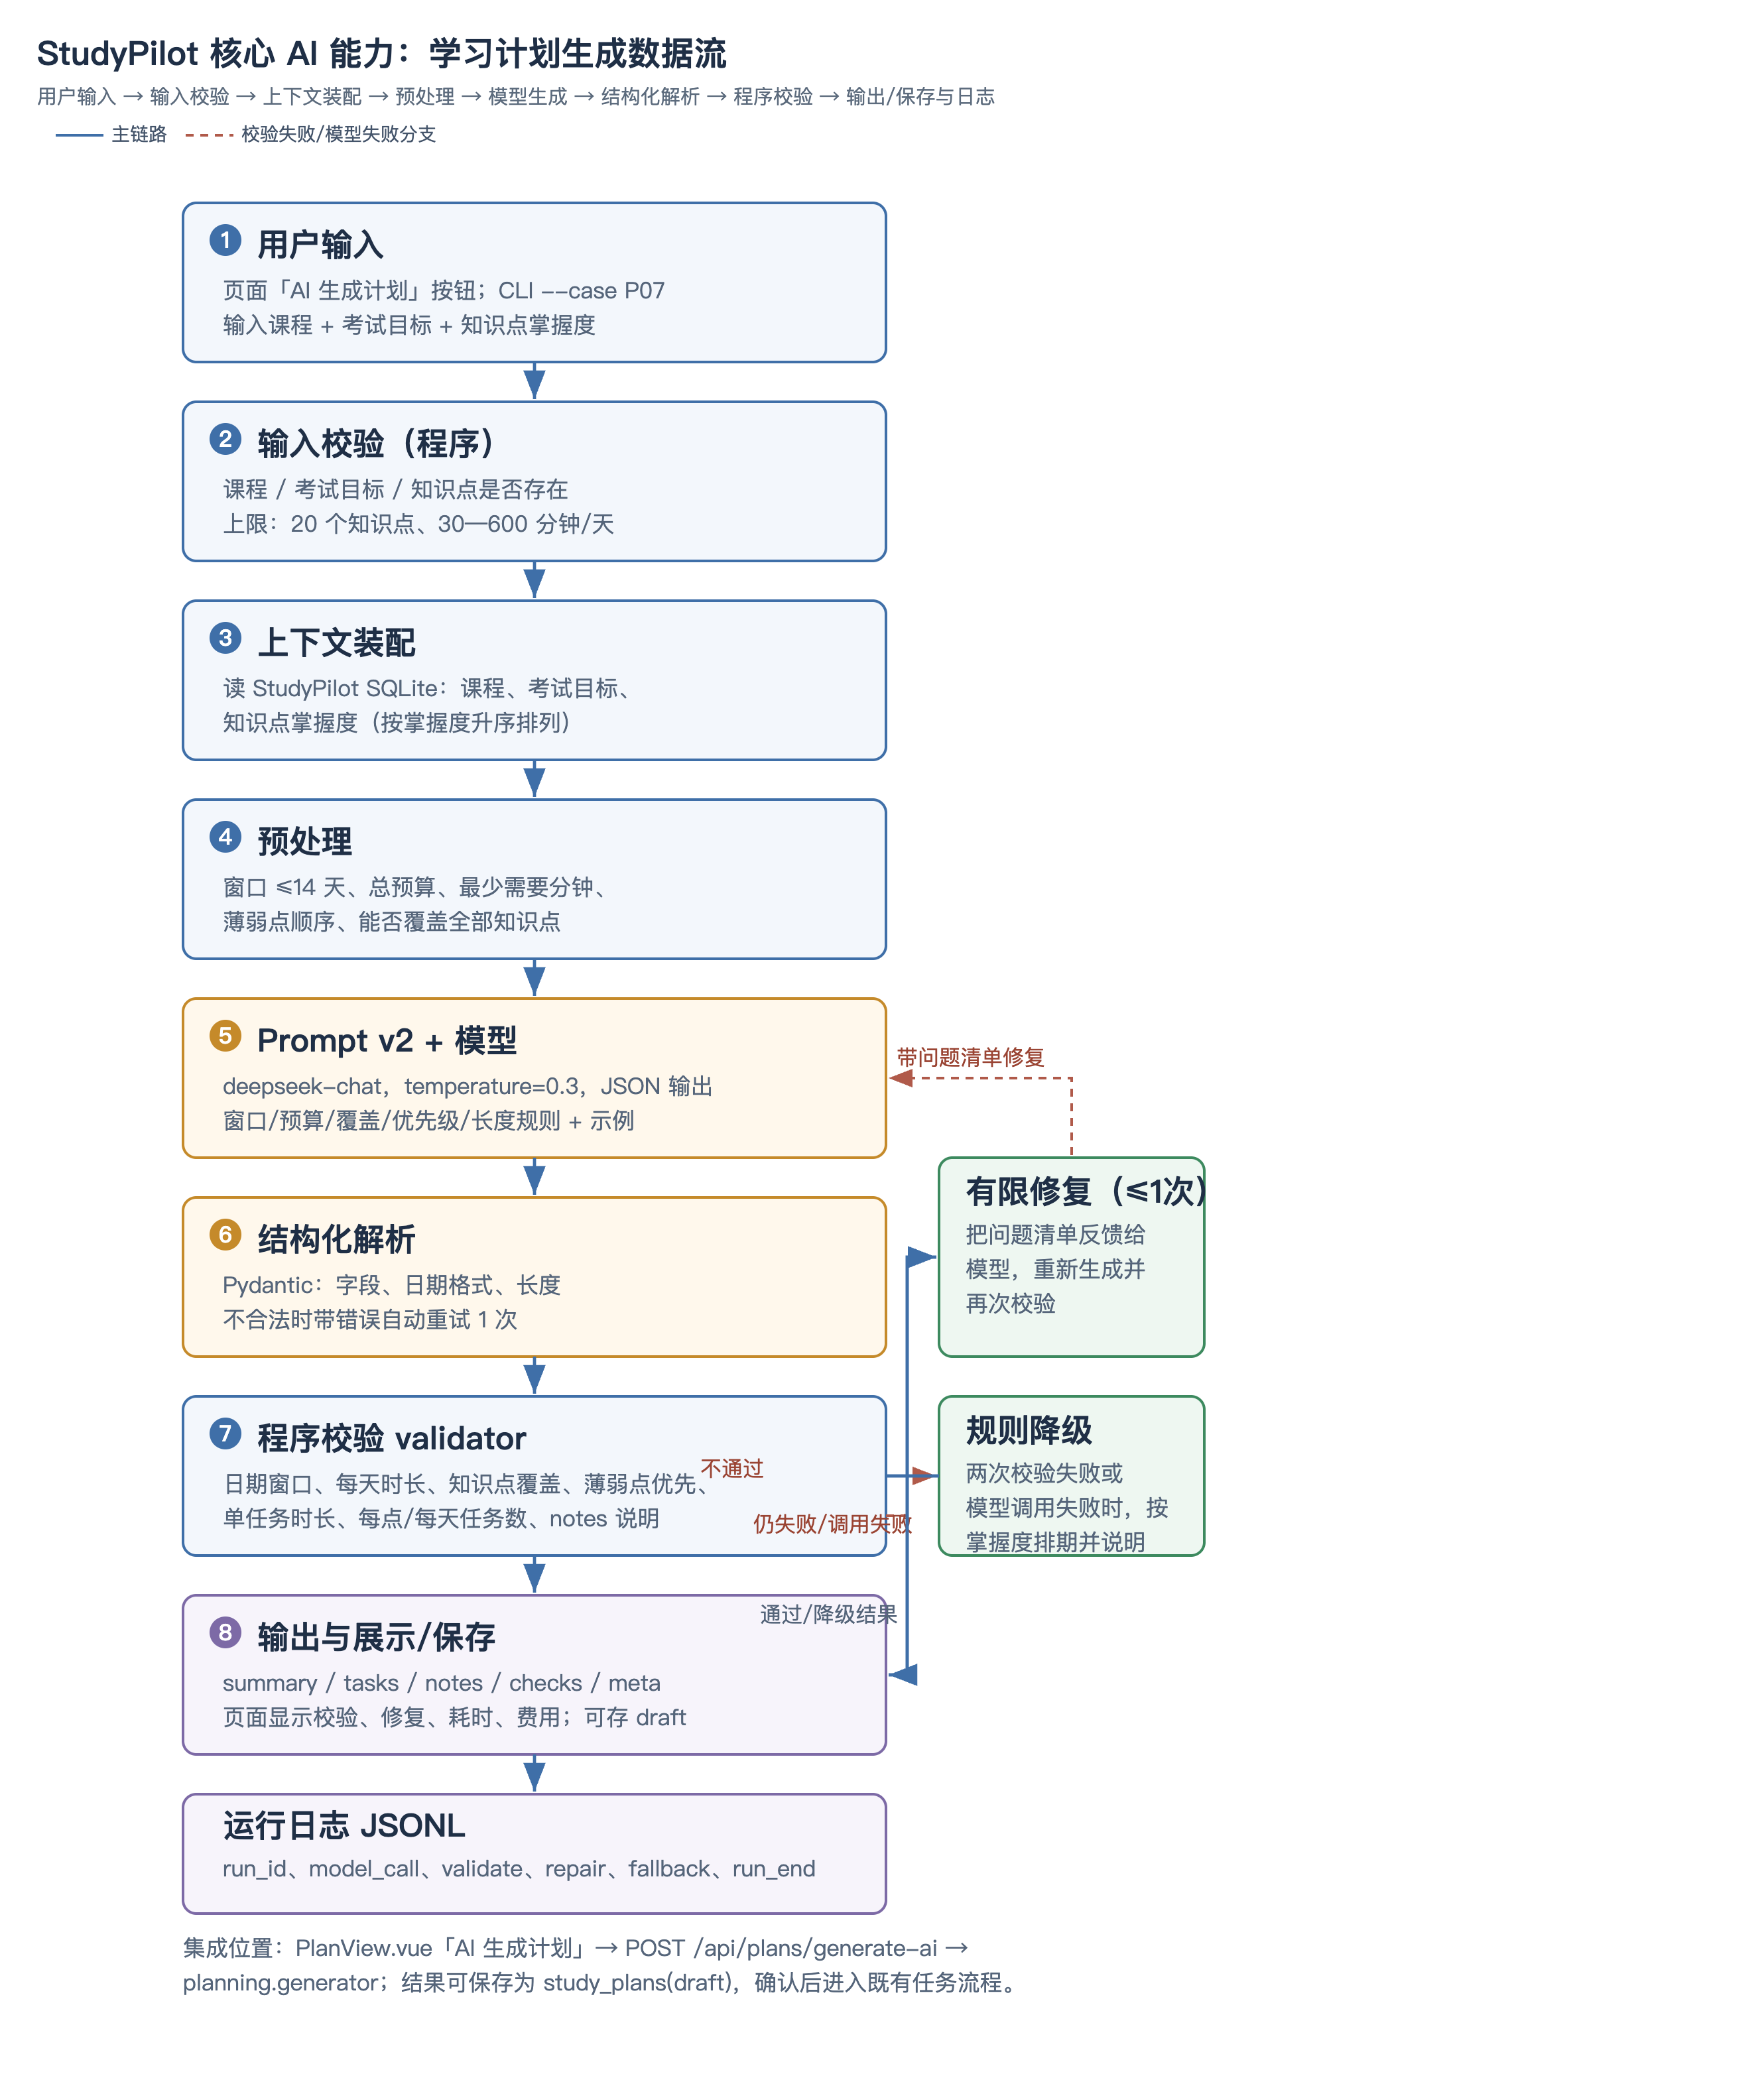
\includegraphics[width=0.79\textwidth]{e7-flow.png}
\caption{核心AI能力原型数据流：输入、预处理、模型、校验/修复/降级、输出与日志}
\label{fig:flow}
\end{figure}

技术组合只采用一次模型调用，没有引入 RAG、工具调用或 Agent。理由如下。第一，本任务的输入是项目数据库中的结构化数据（课程、考试目标、知识点掌握度、每天可用时间），不存在需要检索的外部资料，用 RAG 反而增加无关上下文。第二，任务是单次生成而非多步决策，模型不需要根据中间结果改变下一步，工具循环和 Agent 只会增加延迟与不确定性。第三，真正的可靠性问题不在“调用多少次模型”，而在“模型输出是否满足业务约束”，因此把工程重点放在程序校验、有限修复和规则降级上。模型通过现有 \texttt{llm\_client.chat\_json} 调用 DeepSeek 的 chat completions 接口，要求 JSON 输出并用 Pydantic 校验结构；没有微调，也没有把密钥写入代码。

模型名称、Prompt 版本、温度、输出上限、超时、修复次数、规模限制和价格都集中在 \texttt{backend/app/planning/config.py}，见表\ref{tab:config}。换模型或比较 Prompt 时只改配置模块，不需要在业务代码中搜索参数。密钥只从环境变量 \texttt{DEEPSEEK\_API\_KEY} 读取；日志写入前对 \texttt{sk-} 前缀做遮挡。

\begin{table}[H]
\centering
\caption{原型主要配置（backend/app/planning/config.py）}
\label{tab:config}
\small
\begin{tabularx}{\textwidth}{L{3.4cm}L{3.2cm}X}
\toprule
配置项 & 取值 & 说明 \\
\midrule
模型 & deepseek-chat & 请求模型；接口实际返回 \texttt{deepseek-flash}，按返回记录 \\
Prompt 版本 & v2（默认），v1 保留 & v2 用于修订版；v1 作为初版对照路径 \\
temperature & 0.3 & 同一输入多次运行仍有差异，评测时如实记录 \\
max\_tokens & 2000 & 初版曾因 1200 截断 JSON，调整后写入 v0.5 配置 \\
单次模型超时 & 45 秒 & httpx 超时；失败后 v0.6 降级，v0.5 直接报错 \\
修复次数 & 1 次 & 第二次输出仍不合格则降级 \\
计划窗口 & $\le$ 14 天 & 从开始日期到考试前一天，最多 14 天 \\
规模限制 & 知识点 $\le$ 20 个 & 超出时在调用模型前拒绝并建议拆分 \\
每天可用 & 30—600 分钟 & 低于 30 分钟或高于 600 分钟拒绝 \\
任务约束 & 10—120 分钟/任务；$\le$ 3 个/天；$\le$ 2 个/知识点 & 由 validator 程序检查，不依赖提示词 \\
估算价格 & 输入 2 元/百万 tokens，输出 8 元/百万 tokens & 按 DeepSeek 官网价格估算，仅用于比较费用 \\
密钥 & DEEPSEEK\_API\_KEY 环境变量 & 不写入代码、命令行参数和仓库 \\
\bottomrule
\end{tabularx}
\end{table}

模块分工见表\ref{tab:modules}。原型没有拆成独立服务，命令行、页面和评测脚本调用同一个 \texttt{generator.generate}。

\begin{table}[H]
\centering
\caption{原型模块分工}
\label{tab:modules}
\scriptsize
\begin{tabularx}{\textwidth}{L{3.6cm}X L{3.2cm}}
\toprule
模块 & 职责 & 关键函数/类 \\
\midrule
\texttt{planning/config.py} & 模型、Prompt、温度、超时、修复次数、规模限制、价格、评测路径 & 常量配置 \\
\texttt{planning/context.py} & 读数据库、输入校验、窗口/预算/可行性计算、提示词上下文 & \texttt{load\_input}、\texttt{prompt\_context} \\
\texttt{planning/prompts.py} & v1 初版 Prompt、v2 约束 Prompt 和边界示例 & \texttt{plan\_messages} \\
\texttt{planning/schema.py} & 模型输出的 Pydantic 结构：字段、日期格式、长度 & \texttt{PlanOut}、\texttt{PlanTaskOut} \\
\texttt{planning/validator.py} & 业务约束校验：日期、时长、覆盖、优先级、任务数、notes & \texttt{validate\_plan}、\texttt{format\_issues} \\
\texttt{planning/generator.py} & 主链路：模型调用、校验、修复、降级、保存 & \texttt{generate}、\texttt{\_run\_v2}、\texttt{rule\_fallback} \\
\texttt{planning/runlog.py} & JSONL 运行日志、运行编号、密钥遮挡 & \texttt{RunLogger}、\texttt{new\_run\_id} \\
\texttt{service/llm\_client.py} & 复用实验5的模型调用：超时、错误分类、JSON 重试 & \texttt{chat\_json} \\
\texttt{tools/plan\_ai\_cli.py} & 命令行入口；\texttt{--case} 可复现评测样例 & \texttt{main} \\
\texttt{tools/plan\_eval.py} & 对同一评测集运行规则/v0.5/v0.6，汇总指标 & \texttt{run\_case}、\texttt{summarize} \\
\texttt{tools/plan\_checks.py} & 评测用独立检查器，不依赖生成器内部判断 & \texttt{check\_plan}、\texttt{is\_feasible} \\
\texttt{tools/plan\_log.py} & 按运行编号查看 JSONL 日志 & \texttt{main} \\
\texttt{api/plans.py} & \texttt{POST /api/plans/generate-ai} 接口 & \texttt{generate\_ai} \\
\texttt{web/src/views/PlanView.vue} & 页面按钮、校验结果、修复次数、费用与任务表 & \texttt{generateAI} \\
\texttt{tests/test\_planning.py} & 20 个离线用例：输入、校验、修复、降级、保存、接口 & 见 3.5 \\
\bottomrule
\end{tabularx}
\end{table}

与基础软件的连接位置有两处：生成结果是候选计划，命令行 \texttt{--save} 或接口 \texttt{save=True} 会保存为 \texttt{study\_plans(draft)} 和 \texttt{daily\_tasks}；页面“确认计划”走实验4已有的 \texttt{/api/plans/confirm}，保存为正式计划并进入任务流程（该接口目前仍把 generator 记为 rule\_template，尚未把 AI 生成方式传过去，是集成遗留）；接口 \texttt{POST /api/plans/generate-ai} 接收 \texttt{course\_id}、可选的 \texttt{available\_minutes}、\texttt{start\_date}、\texttt{save}，返回 \texttt{tasks}、\texttt{summary}、\texttt{notes}、\texttt{checks} 和 \texttt{meta}。本次只做到页面入口与 draft 保存，不把生成过程嵌入任务完成或进度更新。

\subsection*{3.4 端到端主链路实现}

一次正常生成的主链路如下：
\begin{enumerate}[leftmargin=2.4em,itemsep=0.15em]
  \item 用户在“学习计划”页选择课程后点击“AI 生成计划”，或在命令行执行 \texttt{python3 -m app.tools.plan\_ai\_cli --course 软件工程 --version v2}；
  \item \texttt{load\_input} 读取课程、考试目标、知识点，校验信息是否完整、考试日期是否晚于今天、知识点数量和每天可用时间是否在上限内；
  \item 程序计算计划窗口（最多 14 天）、总预算、最少需要分钟、薄弱点顺序和“能否覆盖全部知识点”；
  \item 由程序拼装 v2 Prompt，调用模型；Prompt 中明确窗口、每天上限、覆盖、优先级、任务数量和输出长度；
  \item 模型返回 JSON 后先用 Pydantic 校验字段和日期格式，再由 validator 逐项检查业务约束；
  \item 不通过时把问题清单反馈给模型修复一次；第二次仍不通过或模型调用失败时，改用规则模板生成并在 \texttt{notes} 中说明降级原因；
  \item 通过后返回任务表、计划说明、取舍说明、校验结果和调用元数据；页面展示，用户修改后确认保存，或命令行 \texttt{--save} 保存为 draft；
  \item 每个关键步骤写入 \texttt{backend/logs/plan\_ai\_runs.jsonl}，包括输入摘要、模型调用、校验、修复、降级和结束状态。
\end{enumerate}

图\ref{fig:v05run} 和 图\ref{fig:v06run} 是同一评测样例 P02（高等数学，3 个知识点，考试距今 16 天，每天 90 分钟）在初版和修订版上的实际输出。初版生成 14 个任务、合计 1260 分钟，每天排满 90 分钟，没有程序校验栏；修订版生成 6 个任务、合计 260 分钟，每个知识点 2 个任务，程序校验通过。两图使用相同的 \texttt{--case P02} 输入，便于直接对比。

\begin{figure}[H]
\centering
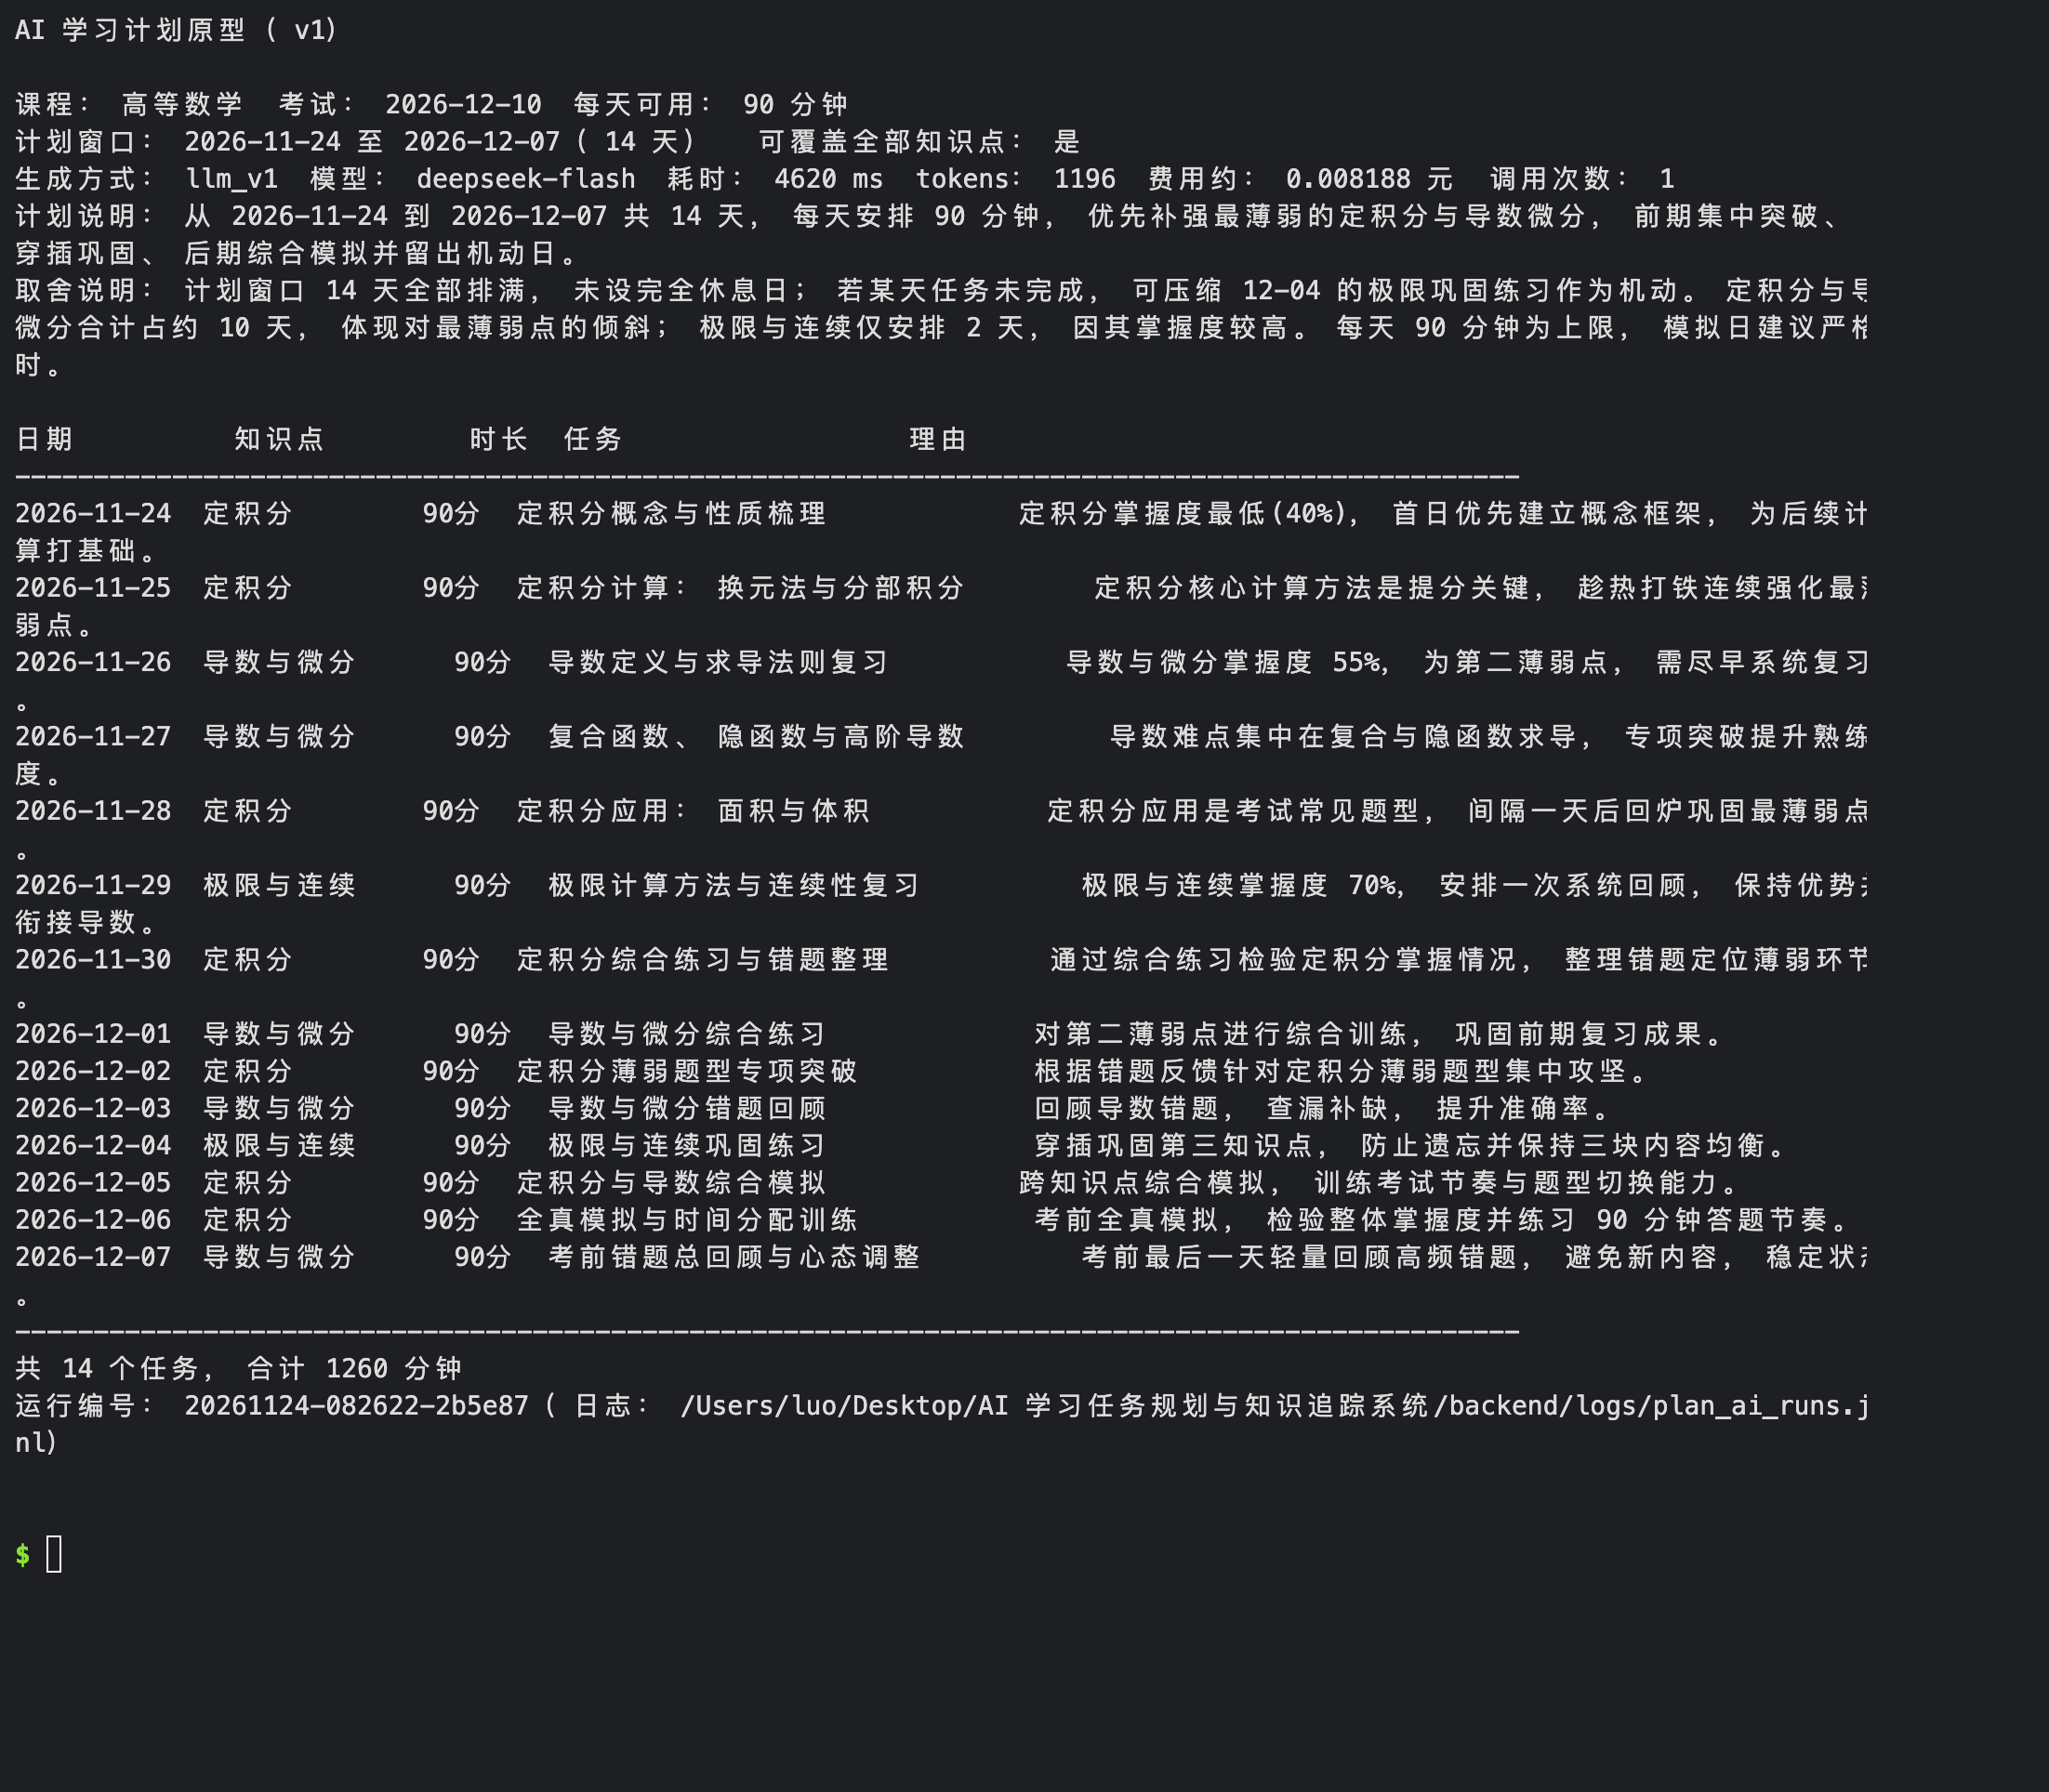
\includegraphics[width=0.94\textwidth]{e7-v05-run.png}
\caption{v0.5 初版：P02 输出 14 个任务、1260 分钟，只有结构校验（4620 ms，1196 tokens，约 0.0082 元）}
\label{fig:v05run}
\end{figure}

\begin{figure}[H]
\centering
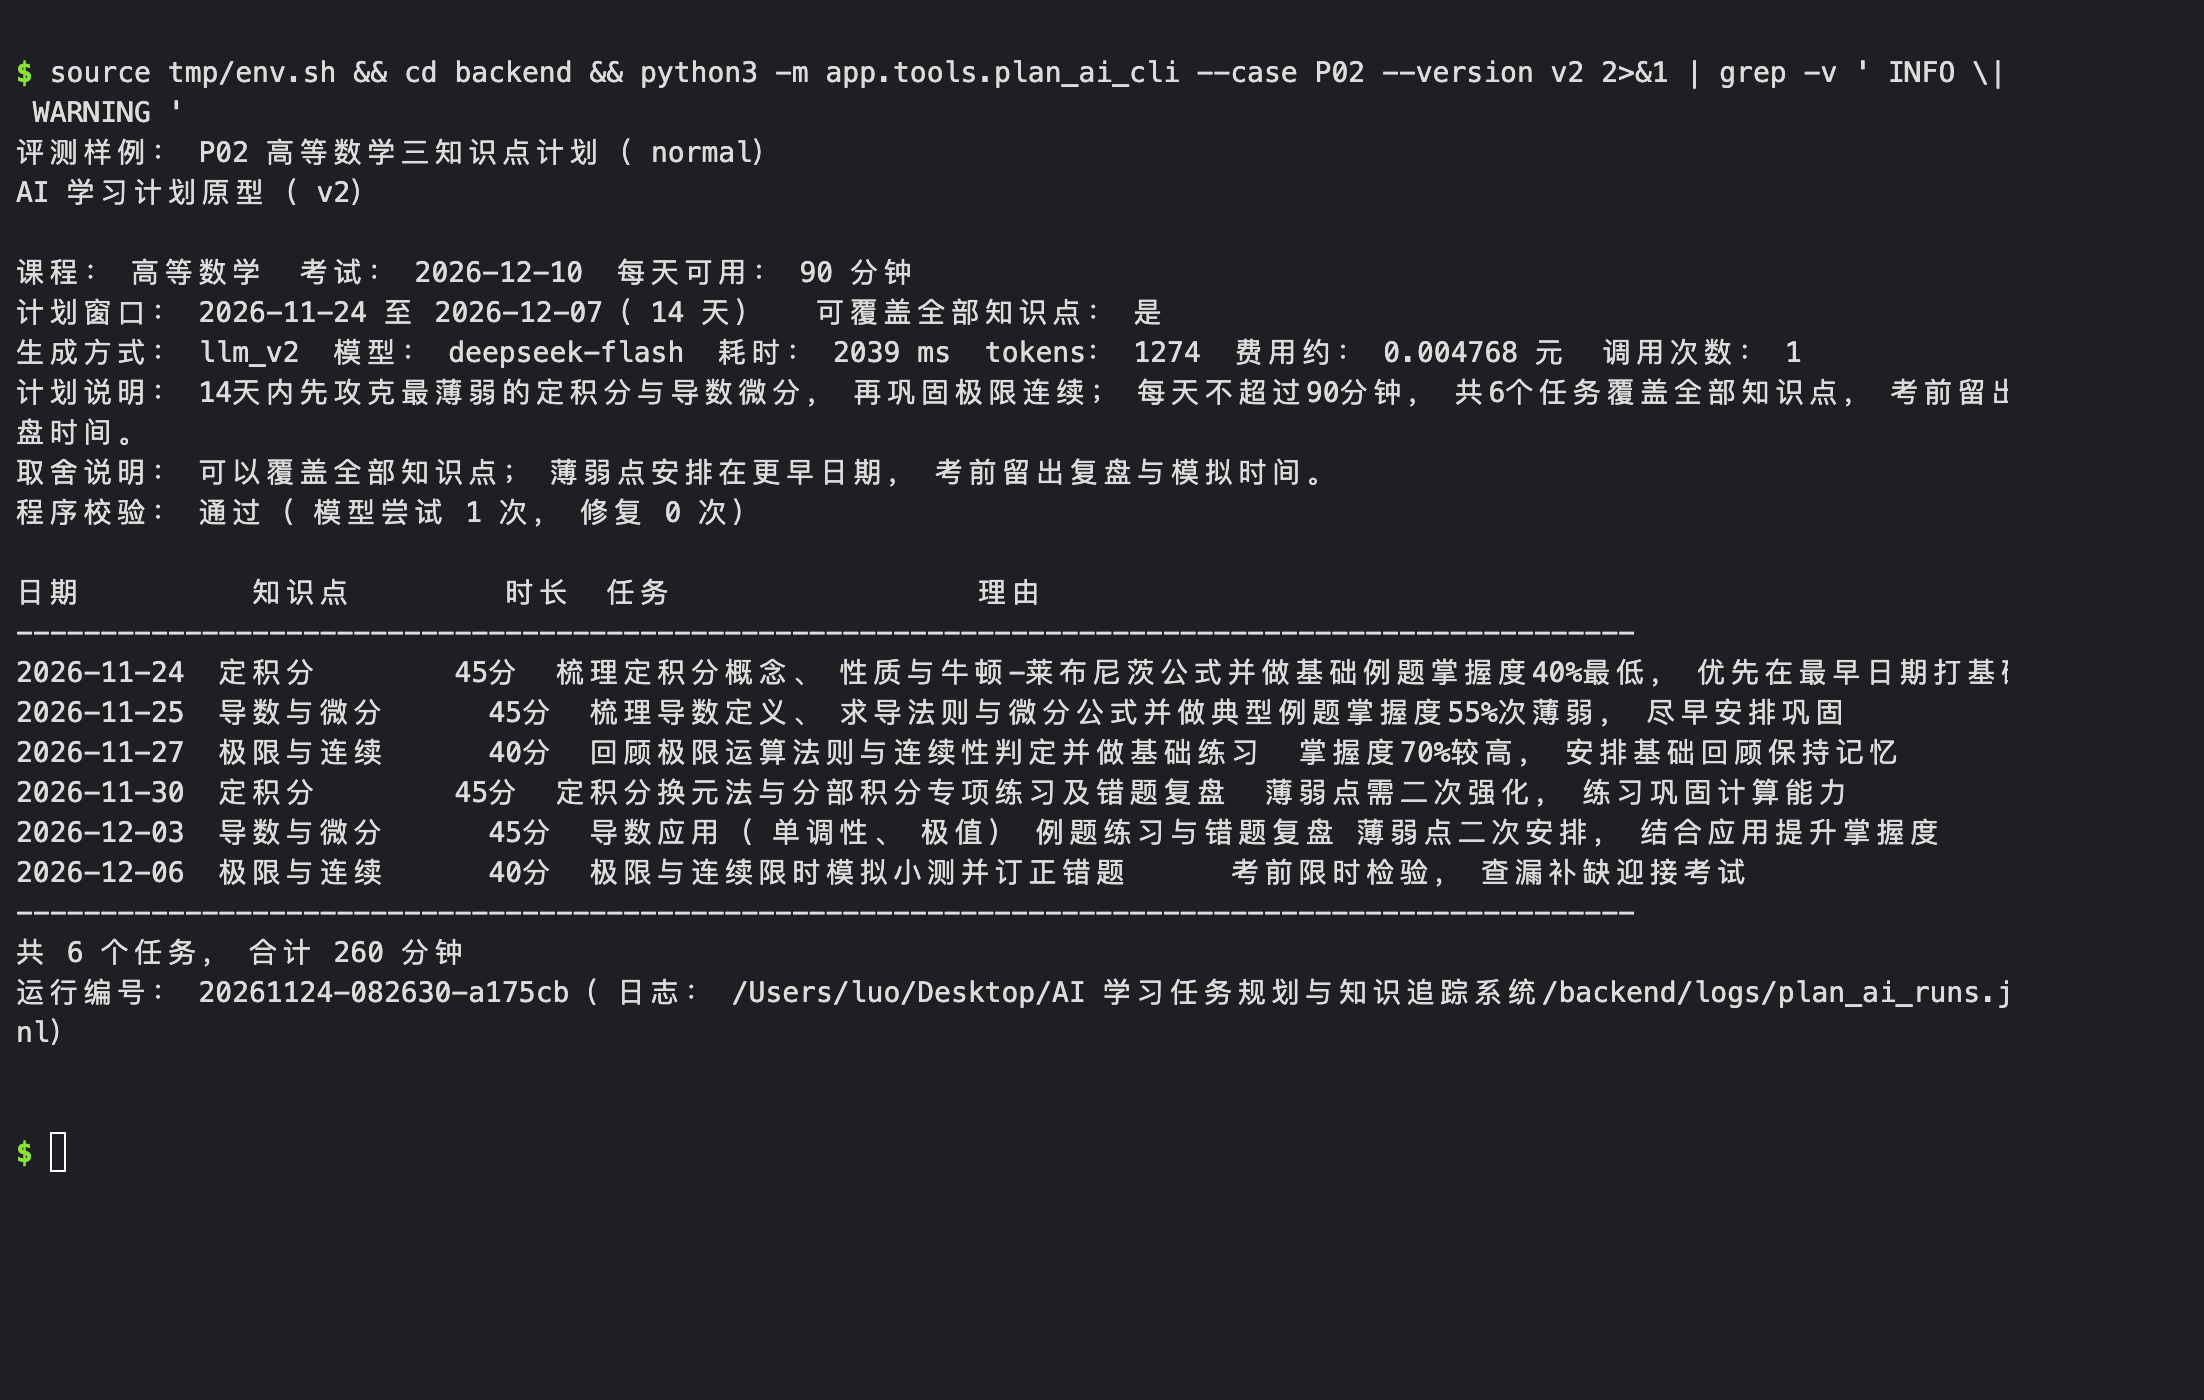
\includegraphics[width=0.94\textwidth]{e7-v06-run.png}
\caption{v0.6 修订版：P02 输出 6 个任务、260 分钟，程序校验通过（2039 ms，1274 tokens，约 0.0048 元）}
\label{fig:v06run}
\end{figure}

页面上的效果见图\ref{fig:ui}：点击“AI 生成计划（带检查）”后，在任务表上方显示生成方式、Prompt 版本、程序校验结果、修复次数、模型调用次数、耗时、tokens 和估算费用，并显示计划说明与取舍说明；任务表仍然可以手工修改，确认按钮走实验4已有的确认接口。

\begin{figure}[H]
\centering
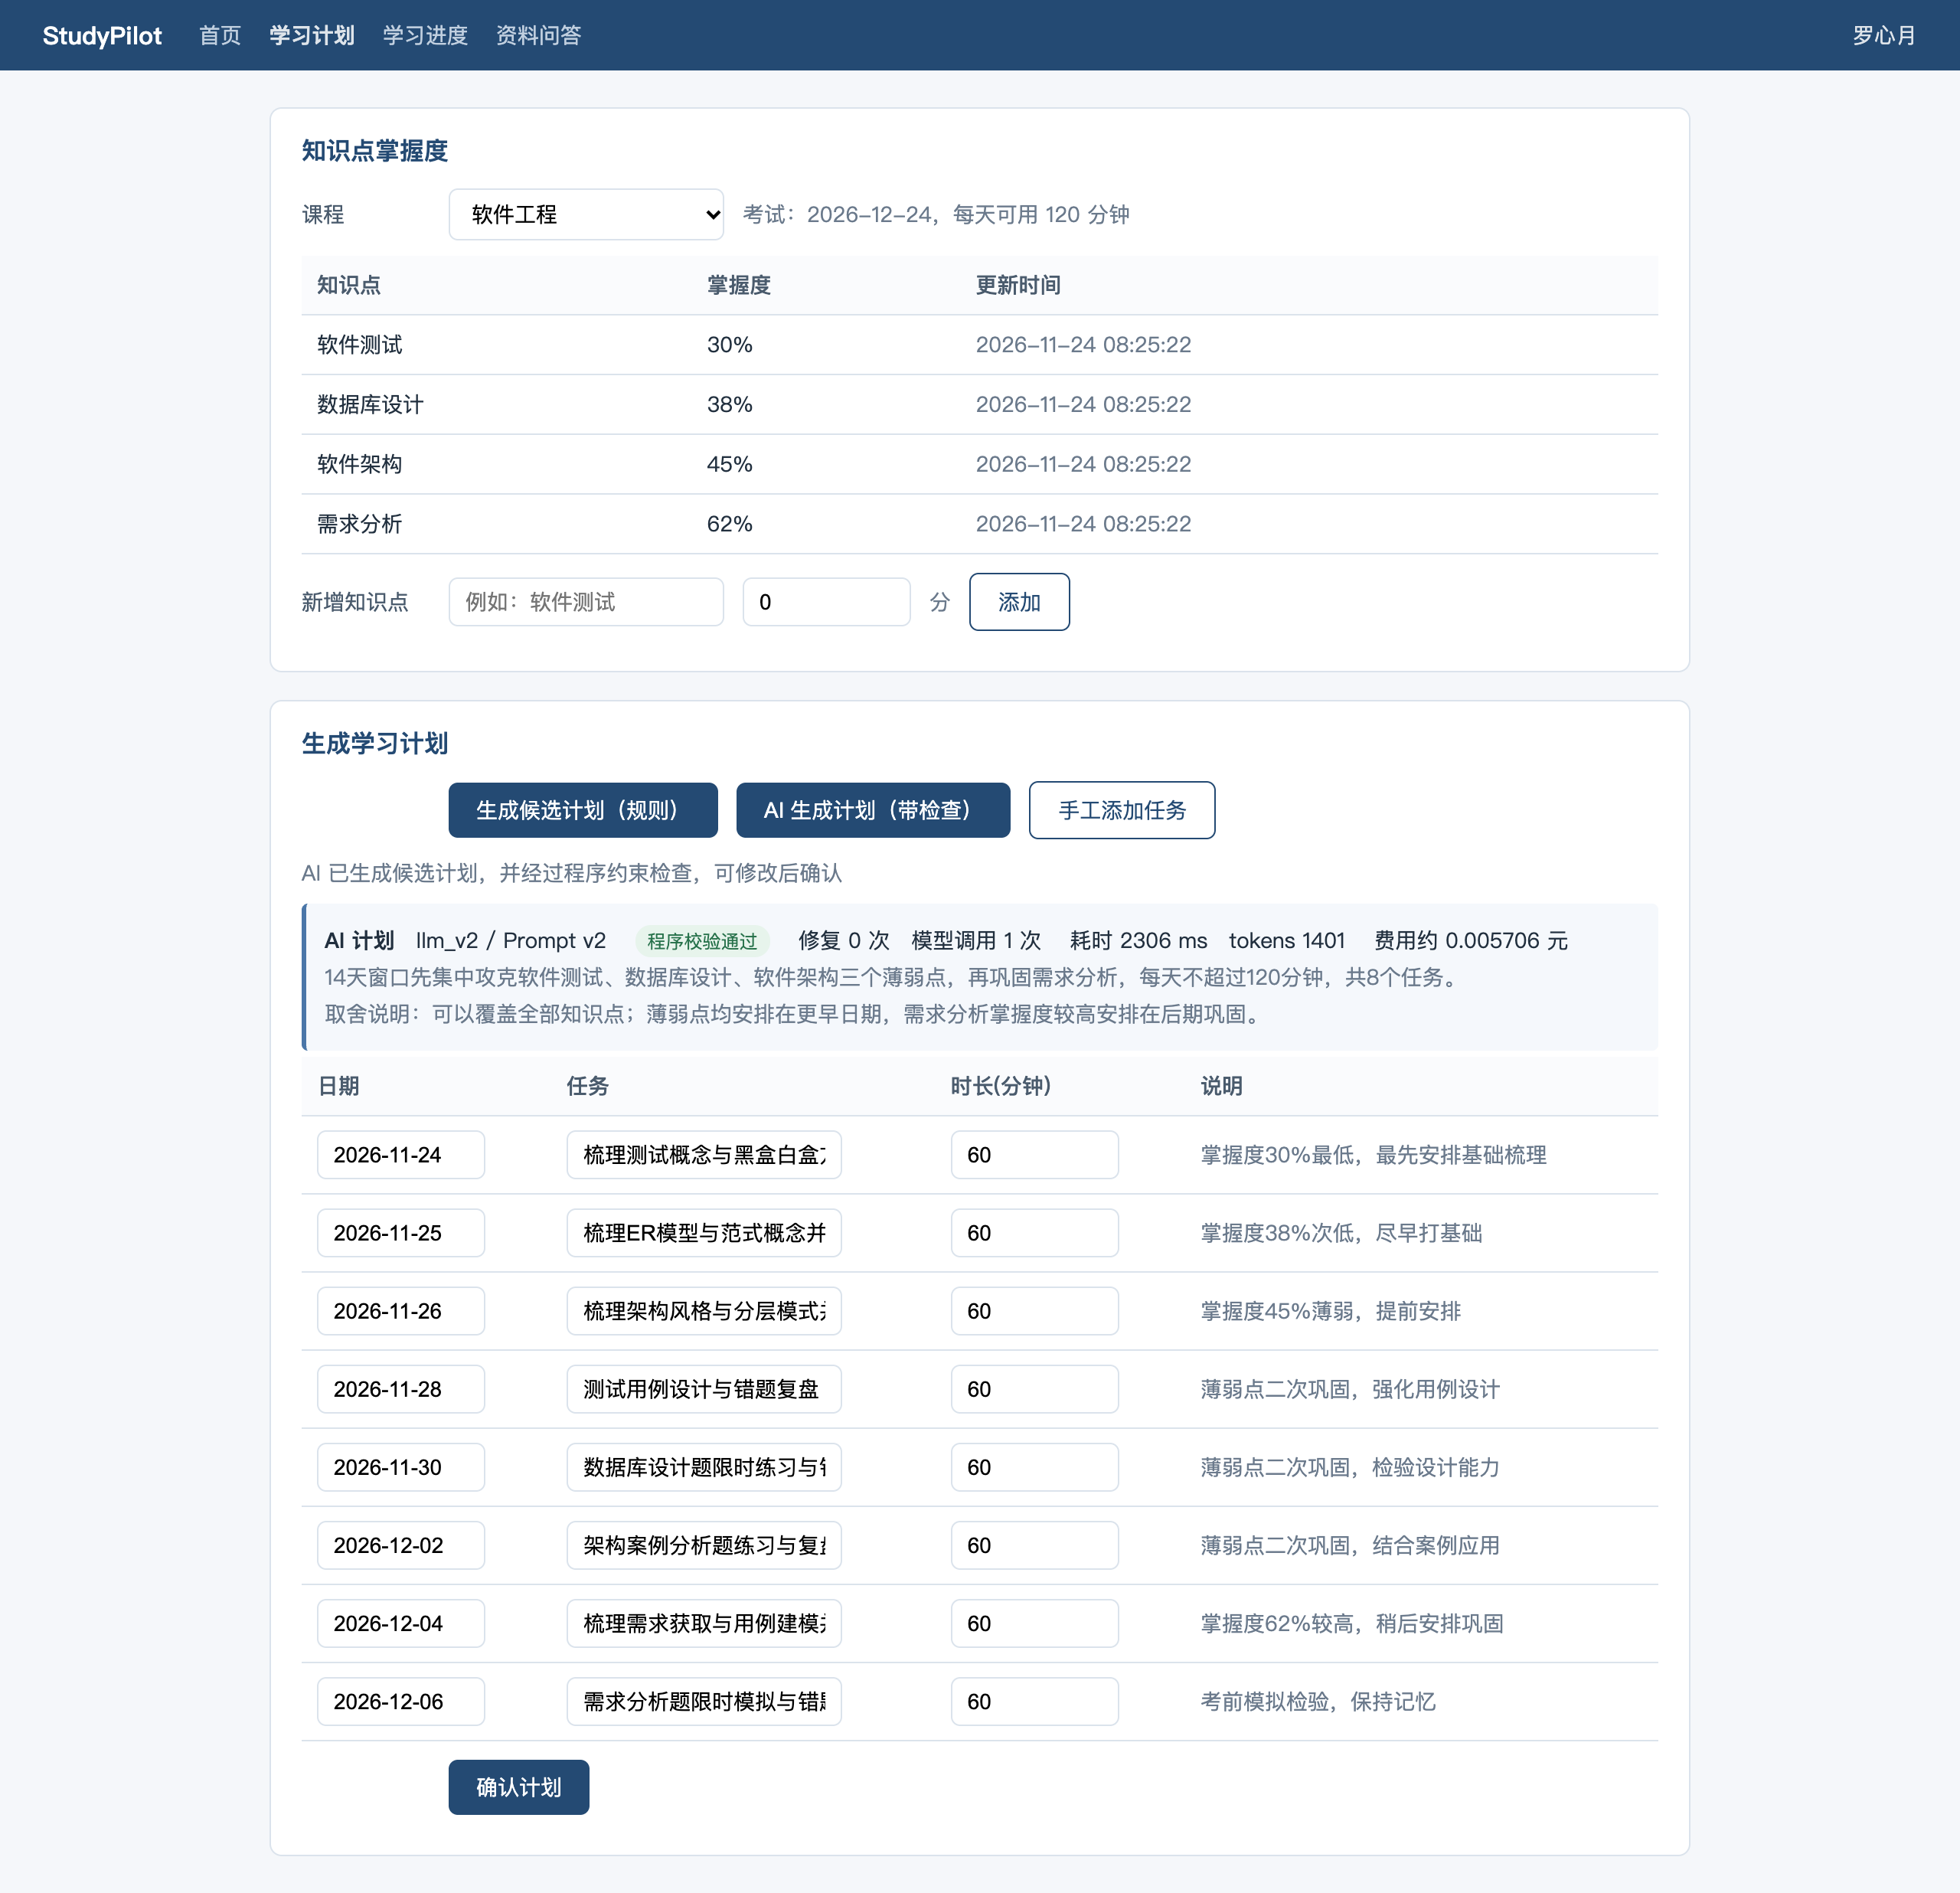
\includegraphics[width=0.86\textwidth]{e7-ui.png}
\caption{学习计划页的 AI 生成入口与结果面板：8 个任务、校验通过、2306 ms、1401 tokens、约 0.0057 元}
\label{fig:ui}
\end{figure}

图\ref{fig:reject} 是两个输入不足/超出范围的场景：P11 没有考试目标，P13 考试日期已过。两者都在调用模型前返回明确错误码和可操作提示，不会生成无效计划，也不消耗模型调用。

\begin{figure}[H]
\centering
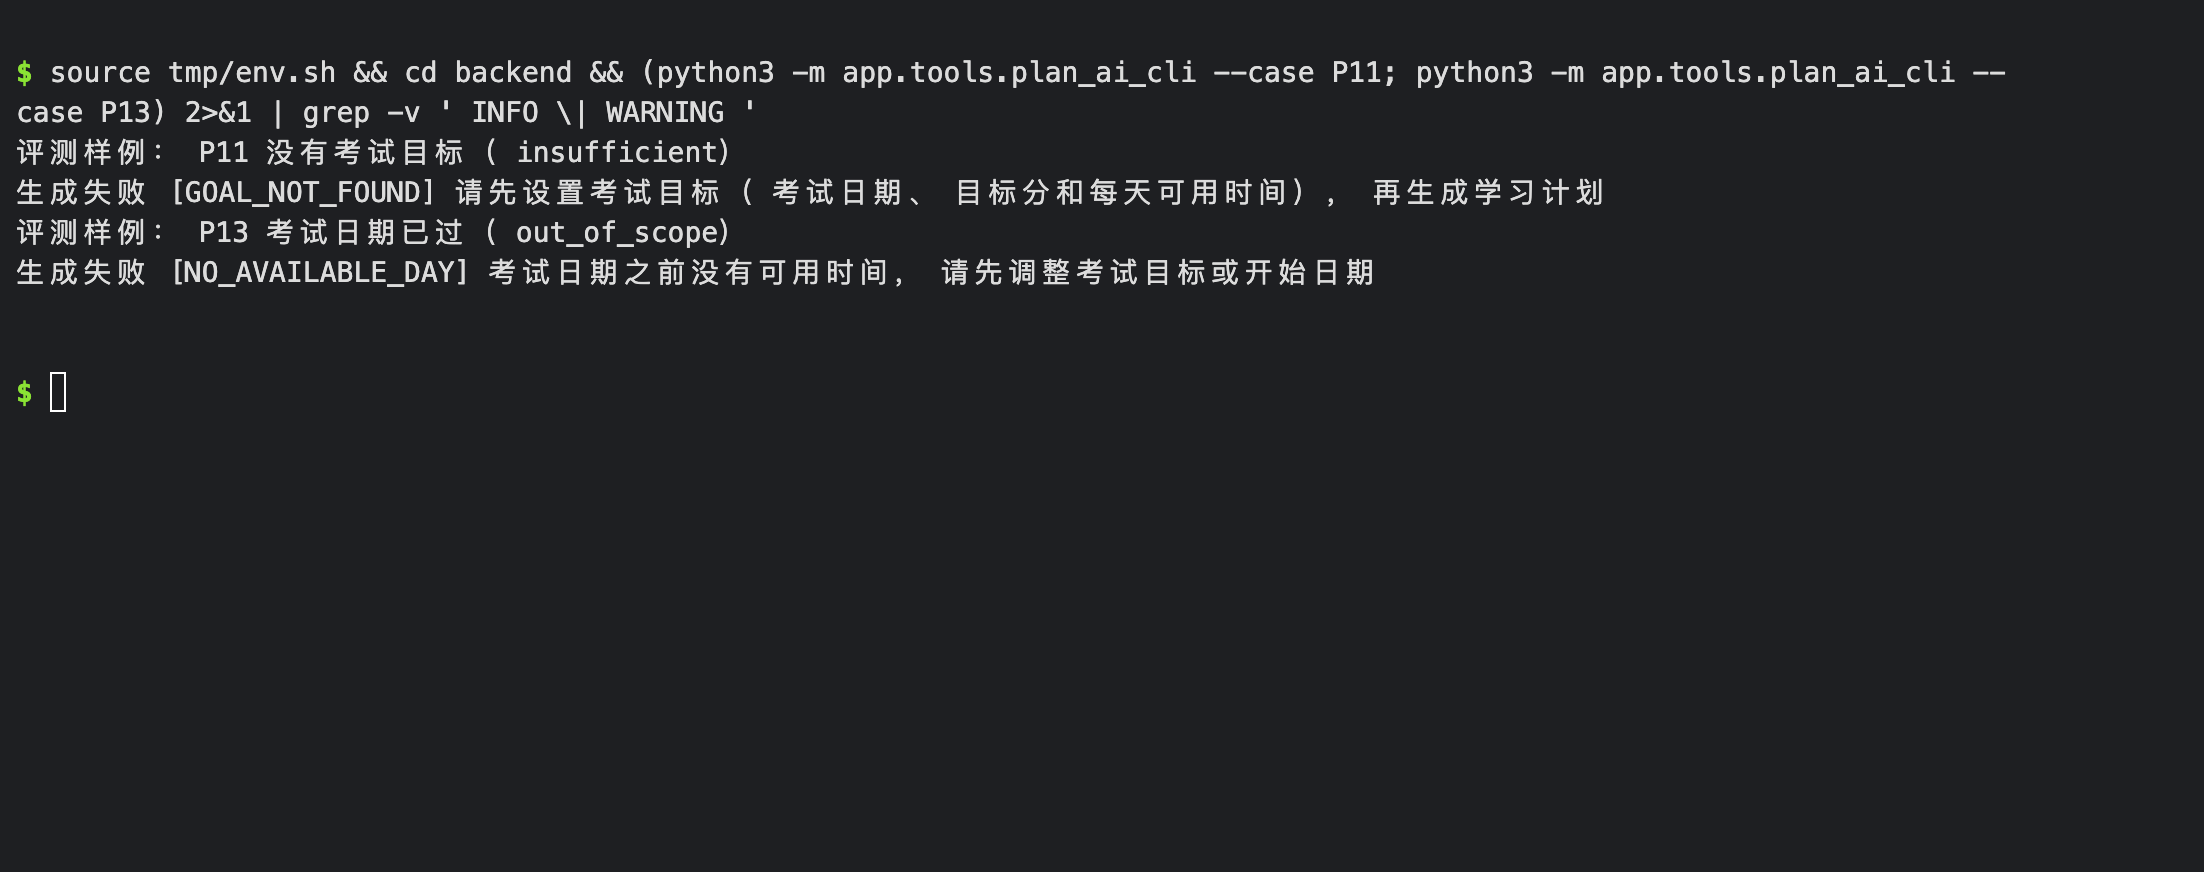
\includegraphics[width=0.92\textwidth]{e7-reject.png}
\caption{输入校验：缺少考试目标、考试日期已过，均在调用模型前拒绝并给出错误码与提示}
\label{fig:reject}
\end{figure}

图\ref{fig:log} 是 P07 的一次真实运行日志。第一次模型输出在 2026-11-24 安排了 4 个任务，validator 判为 \texttt{TOO\_MANY\_TASKS\_PER\_DAY}；程序把问题清单反馈给模型后，第二次输出改为 3 个任务、合计 120 分钟，validator 通过。该运行共 2 次模型调用、2969 tokens、4124 ms，修复 1 次。评测中 9 个可生成样例有 3 个触发修复（P01、P02、P07）：P01 第一次同一知识点排了 3 个任务，P02 第一次任务数超过每点上限，P07 第一次一天排了 4 个任务；修复后全部通过。

\begin{figure}[H]
\centering
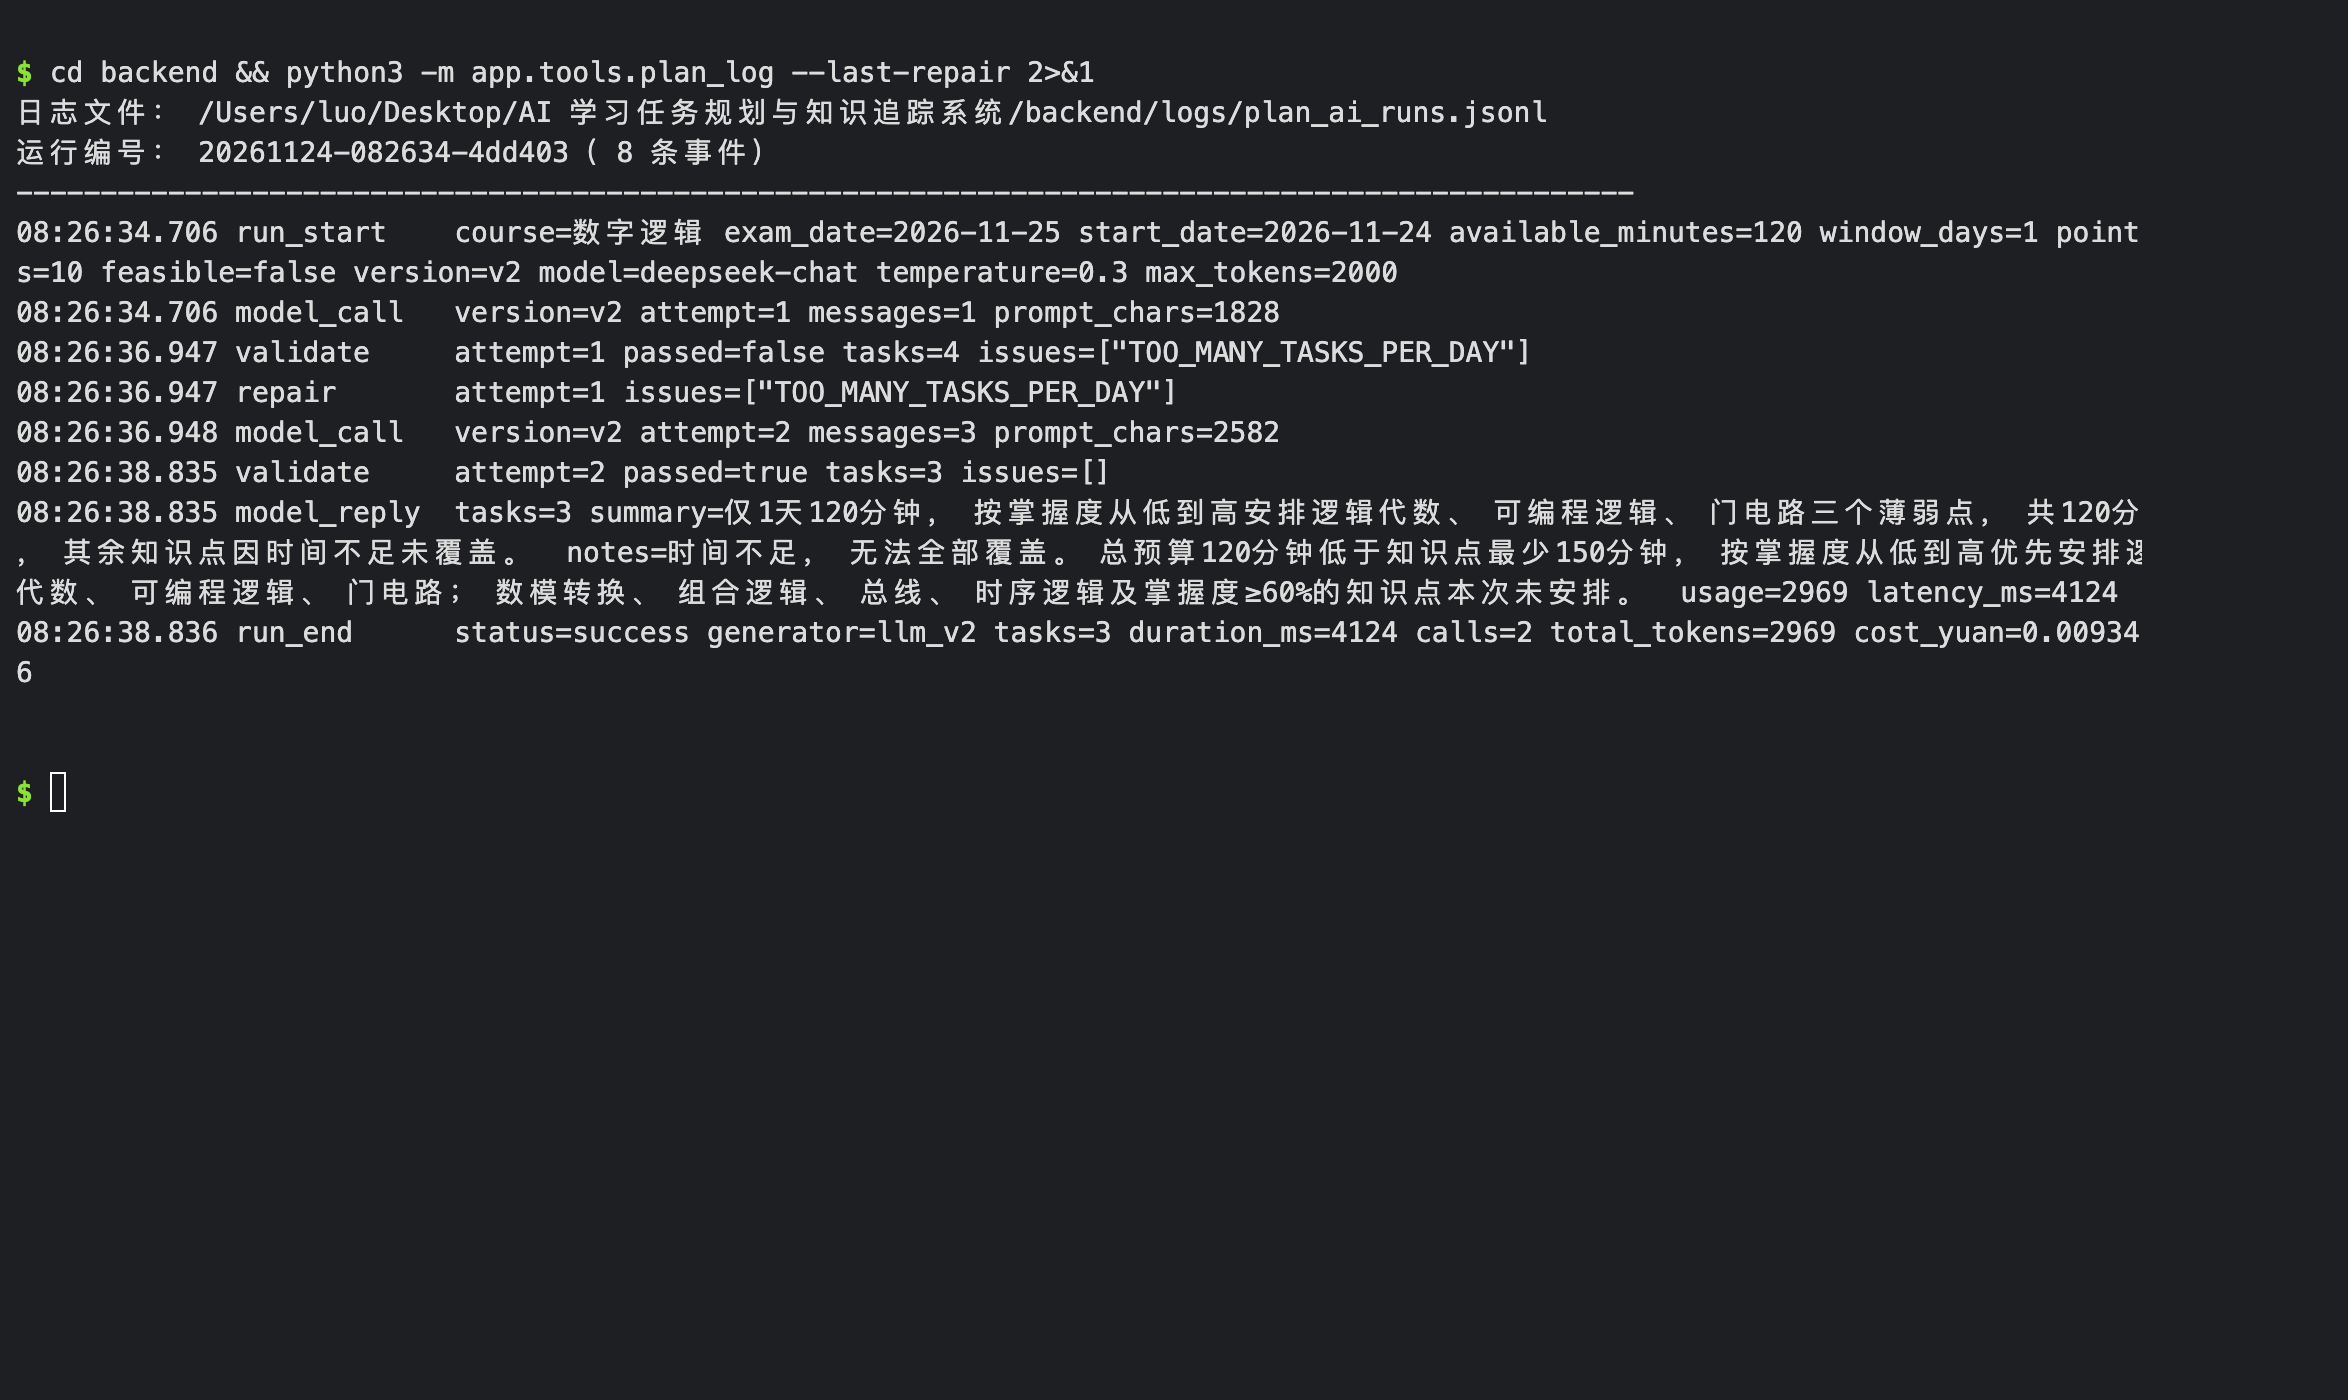
\includegraphics[width=0.96\textwidth]{e7-log.png}
\caption{运行日志：P07 第一次校验失败（TOO\_MANY\_TASKS\_PER\_DAY），修复后通过（run\_id 20261124-082634-4dd403）}
\label{fig:log}
\end{figure}

模型调用失败或两次校验都不通过时的降级分支见图\ref{fig:fallback}。图中把模型名故意设为不存在的 \texttt{no-such-model}，接口返回 HTTP 400；程序记录 \texttt{LLM\_HTTP\_ERROR}，随后返回规则模板计划（4 个任务、95 分钟）并在“降级原因”中说明，程序校验仍然通过。这样即使模型服务不可用，页面也能拿到可执行计划，而不是空白或报错。

\begin{figure}[H]
\centering
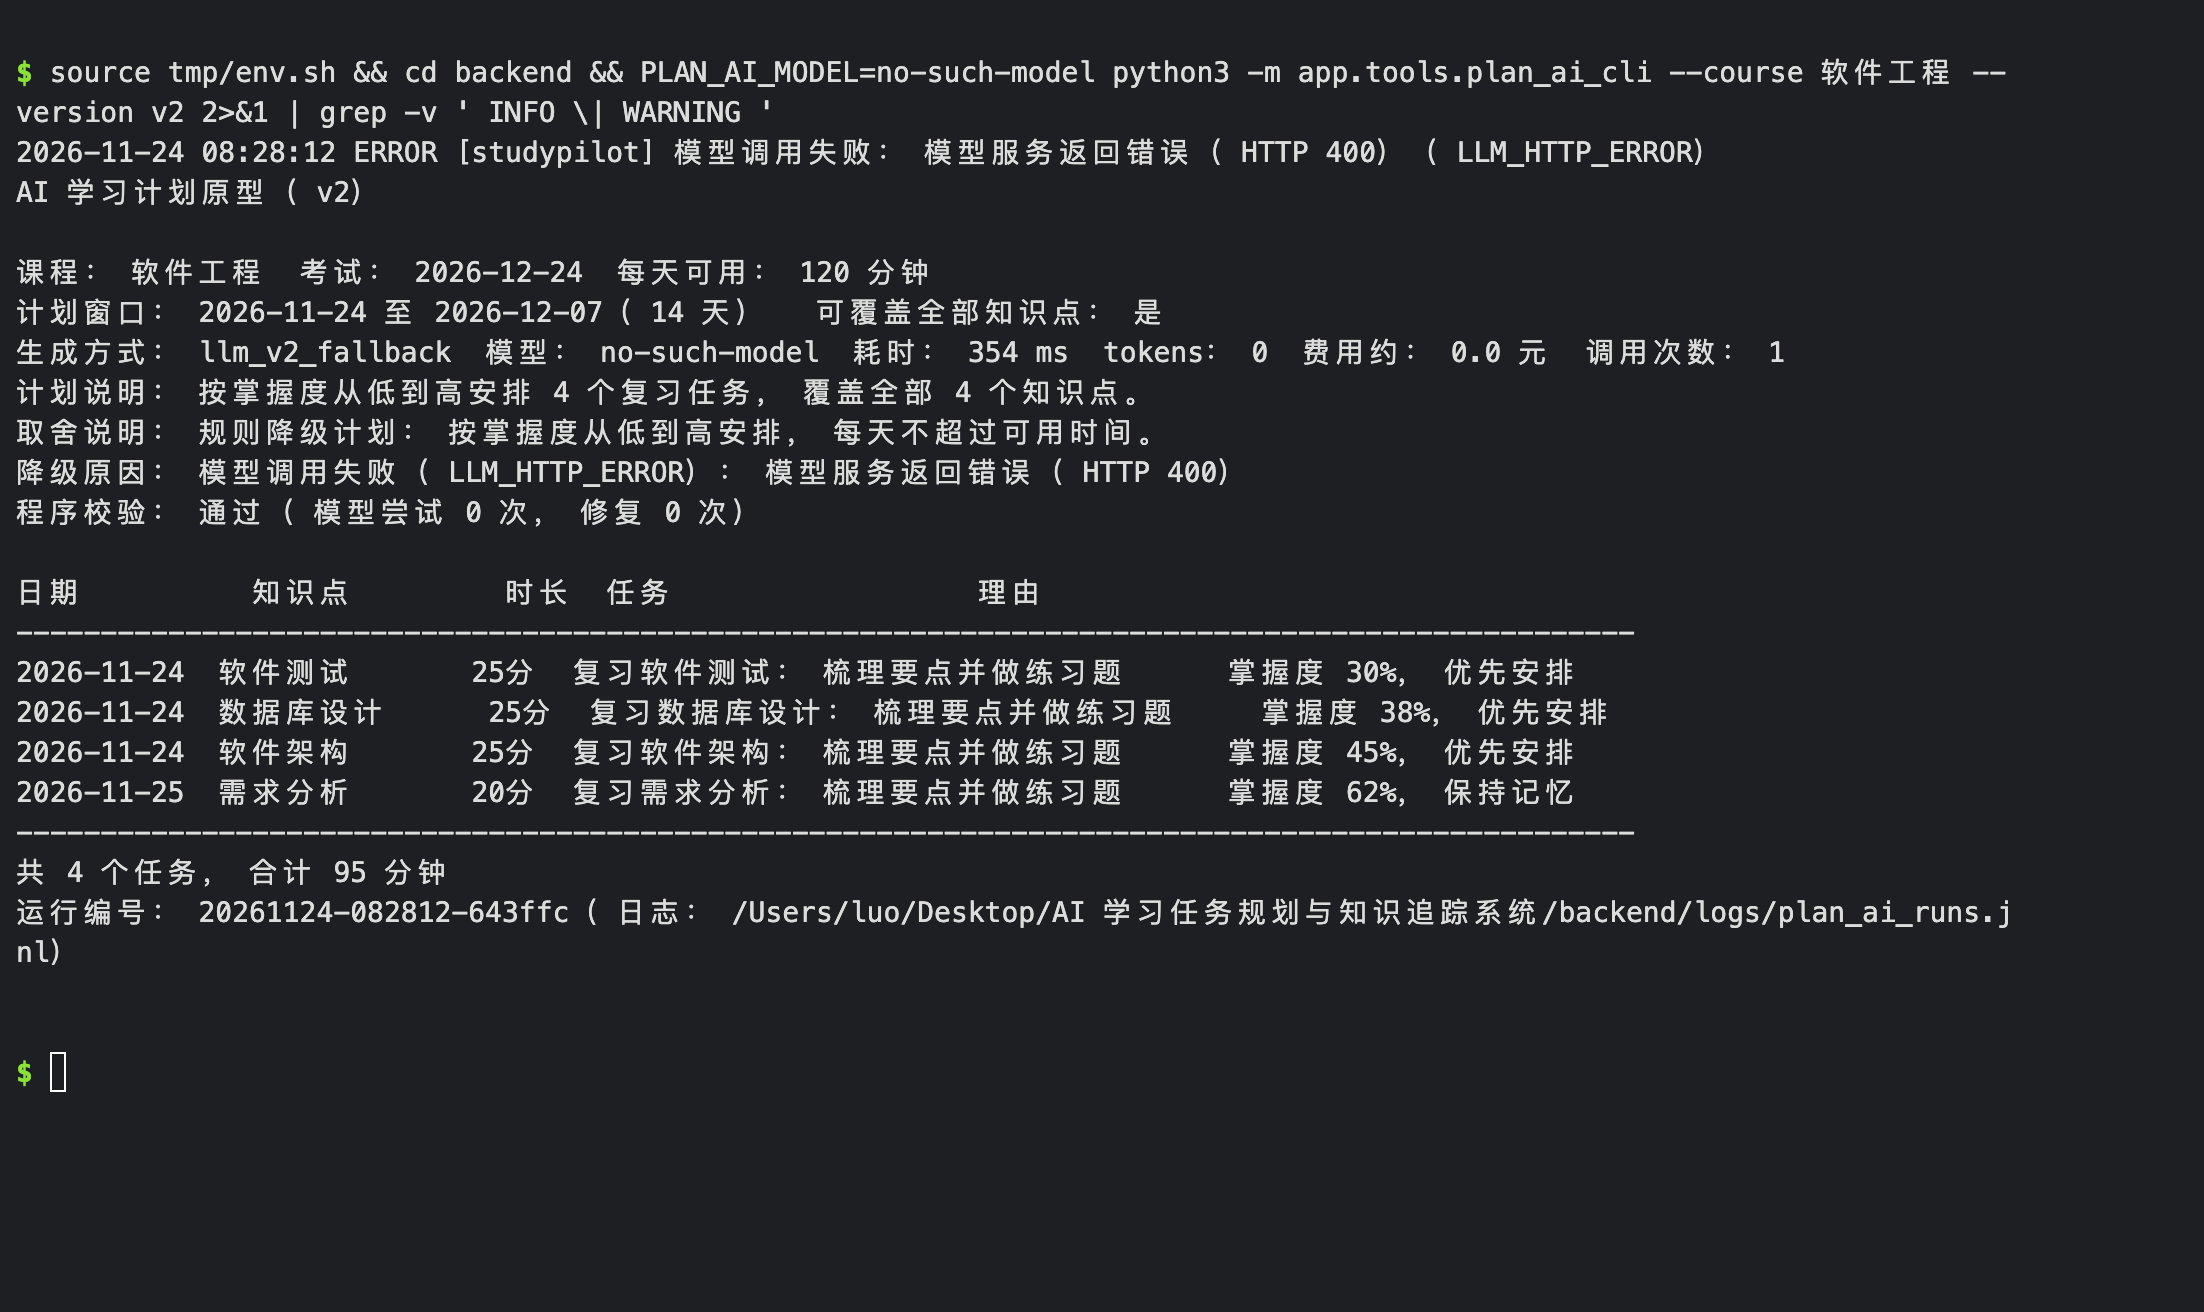
\includegraphics[width=0.94\textwidth]{e7-fallback.png}
\caption{降级分支：模型名错误导致 HTTP 400，自动改用规则模板并说明原因（1 次失败调用被计入）}
\label{fig:fallback}
\end{figure}

运行日志的事件和字段见表\ref{tab:logfields}。每次运行有唯一 \texttt{run\_id}，时间、课程、窗口、限制、每次模型调用、校验结果、修复问题、降级原因和结束状态都可追溯；日志不含密钥，课程名和知识点名来自本人样例数据。失败时可以从 \texttt{validate}、\texttt{llm\_error} 或 \texttt{fallback} 事件判断问题出在模型、参数、校验规则还是降级逻辑，而不是只看一个最终状态。

\begin{table}[H]
\centering
\caption{运行日志事件与主要字段}
\label{tab:logfields}
\small
\begin{tabularx}{\textwidth}{L{2.8cm}X}
\toprule
事件 & 主要字段 \\
\midrule
run\_start & 课程、考试日期、开始日期、每天可用、窗口天数、知识点数、是否可覆盖、版本、模型、温度、max\_tokens \\
model\_call & 版本、第几次尝试、上下文消息数、Prompt 字符数 \\
validate & 第几次尝试、是否通过、任务数、问题码列表 \\
repair & 第几次尝试、问题码列表 \\
llm\_error / fallback & 错误码、错误信息、降级原因、降级后任务数和校验结果 \\
model\_reply & 任务数、summary/notes 摘要、tokens、耗时 \\
run\_end & 状态（success/rejected/fallback）、生成方式、任务数、耗时、调用次数、tokens、费用 \\
\bottomrule
\end{tabularx}
\end{table}

超时和输出不合要求的处理：模型单次超时 45 秒，由 httpx 控制；结构不合法由 \texttt{chat\_json} 带错误重试一次；业务约束不合法由 validator 生成问题清单并修复一次；模型调用失败、结构重试后仍失败、修复后仍失败都进入规则降级。v0.5 没有业务校验和降级，因此同样的模型失败在初版会直接报错：开发初期 1200 的 \texttt{max\_tokens} 曾把 JSON 截断为不完整字符串，触发 \texttt{LLM\_BAD\_JSON}；v0.5 提交时已把上限提高到 2000，但结构重试后仍失败或模型调用失败时仍没有兜底，这是 v0.6 要修复的问题之一。

\subsection*{3.5 原型评测与基线比较}

选择两个基线。基线 B1 是无AI的规则模板（实验4已有实现），代表“不使用模型时软件能做什么”；基线 B2 是 v0.5 初版原型（直接调用模型、只做结构校验），代表“只把模型接进来、不做工程约束”的效果。两个基线与 v0.6 使用同一批 15 个样例、同一输入、同一个独立检查器和同一份人工评分规则。规则基线只有基础校验（课程、考试目标、知识点、日期），P09、P11—P13 会正确拒绝，但 P14 仍会生成 7 个任务、P15 报 \texttt{NO\_TASK\_GENERATED}，错误码与原型不一致，因此拒绝样例不纳入基线正确率，只比较 9 个可生成样例。规则模板沿用实验4的 7 天窗口（\texttt{MAX\_PLAN\_DAYS=7}），原型允许 14 天；这是 P10 规则覆盖失败的原因之一，报告如实说明这一能力差异，不把基线与修订版的全部差异都归因于模型。

表\ref{tab:overall} 是三种方案的总览，表\ref{tab:checkrates} 是逐项检查通过率，表\ref{tab:percase} 是逐样例结果。所有数字来自 2026-11-24 的 \texttt{week2} 统一评测：v0.5 与 v0.6 都在同一进程中重新运行，规则基线也重新生成；人工评分对同一批输出逐条给出。

\begin{table}[H]
\centering
\caption{规则基线、初版与修订版总览}
\label{tab:overall}
\small
\begin{tabularx}{\textwidth}{L{3.4cm}L{1.6cm}L{1.6cm}L{1.5cm}L{1.3cm}L{1.4cm}L{1.3cm}L{1.3cm}}
\toprule
方案 & 生成 & 拒绝 & 平均耗时 & tokens & 费用(元) & 人工可执行 & 人工理由 \\
\midrule
规则模板（无AI） & 6/9 & — & 1 ms & 0 & 0 & 2.00 & 2.22 \\
v0.5 初版（v1） & 7/9 & 6/6 & 4958 ms & 9402 & 0.0611 & 4.00 & 3.56 \\
v0.6 修订版（v2） & 9/9 & 6/6 & 4334 ms & 18587 & 0.0718 & 4.89 & 4.89 \\
\bottomrule
\end{tabularx}
\end{table}

\begin{table}[H]
\centering
\caption{逐项程序检查通过率（可生成样例）}
\label{tab:checkrates}
\small
\begin{tabularx}{\textwidth}{L{3.2cm}L{2.4cm}L{2.4cm}L{2.4cm}X}
\toprule
检查项 & 规则模板 & v0.5 & v0.6 & 说明 \\
\midrule
schema & 9/9 & 8/9 & 9/9 & 字段、日期格式、知识点名称 \\
date & 9/9 & 9/9 & 9/9 & 日期在窗口内且早于考试 \\
daily\_cap & 9/9 & 9/9 & 9/9 & 每天合计不超过可用时间 \\
coverage & 6/7 & 6/7 & 7/7 & 可覆盖时不能漏知识点 \\
priority & 6/6 & 6/6 & 6/6 & 薄弱点平均排期不晚于高掌握度点 \\
minutes & 9/9 & 9/9 & 9/9 & 单个任务 10—120 分钟 \\
capacity & 9/9 & 9/9 & 9/9 & 总时长不超过窗口预算 \\
summary & — & 9/9 & 9/9 & 模型方案必须有计划说明 \\
notes & 0/2 & 2/2 & 2/2 & 不可行时必须说明取舍 \\
\bottomrule
\end{tabularx}
\end{table}

\begin{table}[H]
\centering
\caption{逐样例对比（“—”表示该类样例对基线不适用）}
\label{tab:percase}
\scriptsize
\begin{tabularx}{\textwidth}{L{0.6cm}L{1.5cm}L{2.1cm}L{2.6cm}L{2.6cm}X}
\toprule
编号 & 类别 & 规则模板 & v0.5 & v0.6 & 主要差异/问题 \\
\midrule
P01 & 正常 & 通过 & 通过 & 通过 & v0.6 第一次同点 3 任务，修复后 8 任务 \\
P02 & 正常 & 通过 & 失败（schema） & 通过 & v0.5 出现未给出的“综合复习”；v0.6 用给定 3 点 \\
P03 & 正常 & 通过 & 通过 & 通过 & v0.5 16 个任务过量；v0.6 6 个任务 \\
P04 & 正常 & 通过 & 失败（coverage） & 通过 & v0.5 漏“词汇”；v0.6 覆盖 6/6 \\
P05 & 正常 & 通过 & 通过 & 通过 & 均覆盖 5 点，v0.6 任务更精简 \\
P06 & 正常 & 通过 & 通过 & 通过 & 无薄弱点，priority 不适用 \\
P07 & 边界 & 失败（notes） & 通过 & 通过（修复 1 次） & 规则只排 1 个任务不说明；v0.6 明确 3 个薄弱点 \\
P08 & 边界 & 失败（notes） & 通过 & 通过 & 规则 3 个任务不说明取舍；v0.6 notes 说明预算 \\
P09 & 边界 & N/A & 拒绝正确 & 拒绝正确 & NO\_AVAILABLE\_DAY \\
P10 & 边界 & 失败（coverage） & 通过 & 通过 & 规则漏“优化”；v0.6 覆盖 8/8 \\
P11 & 信息不足 & N/A & 拒绝正确 & 拒绝正确 & GOAL\_NOT\_FOUND \\
P12 & 信息不足 & N/A & 拒绝正确 & 拒绝正确 & EMPTY\_KNOWLEDGE\_POINTS \\
P13 & 超范围 & N/A & 拒绝正确 & 拒绝正确 & NO\_AVAILABLE\_DAY \\
P14 & 超范围 & N/A & 拒绝正确 & 拒绝正确 & TOO\_MANY\_POINTS \\
P15 & 超范围 & N/A & 拒绝正确 & 拒绝正确 & INVALID\_AVAILABLE\_MINUTES \\
\bottomrule
\end{tabularx}
\end{table}

\begin{figure}[H]
\centering
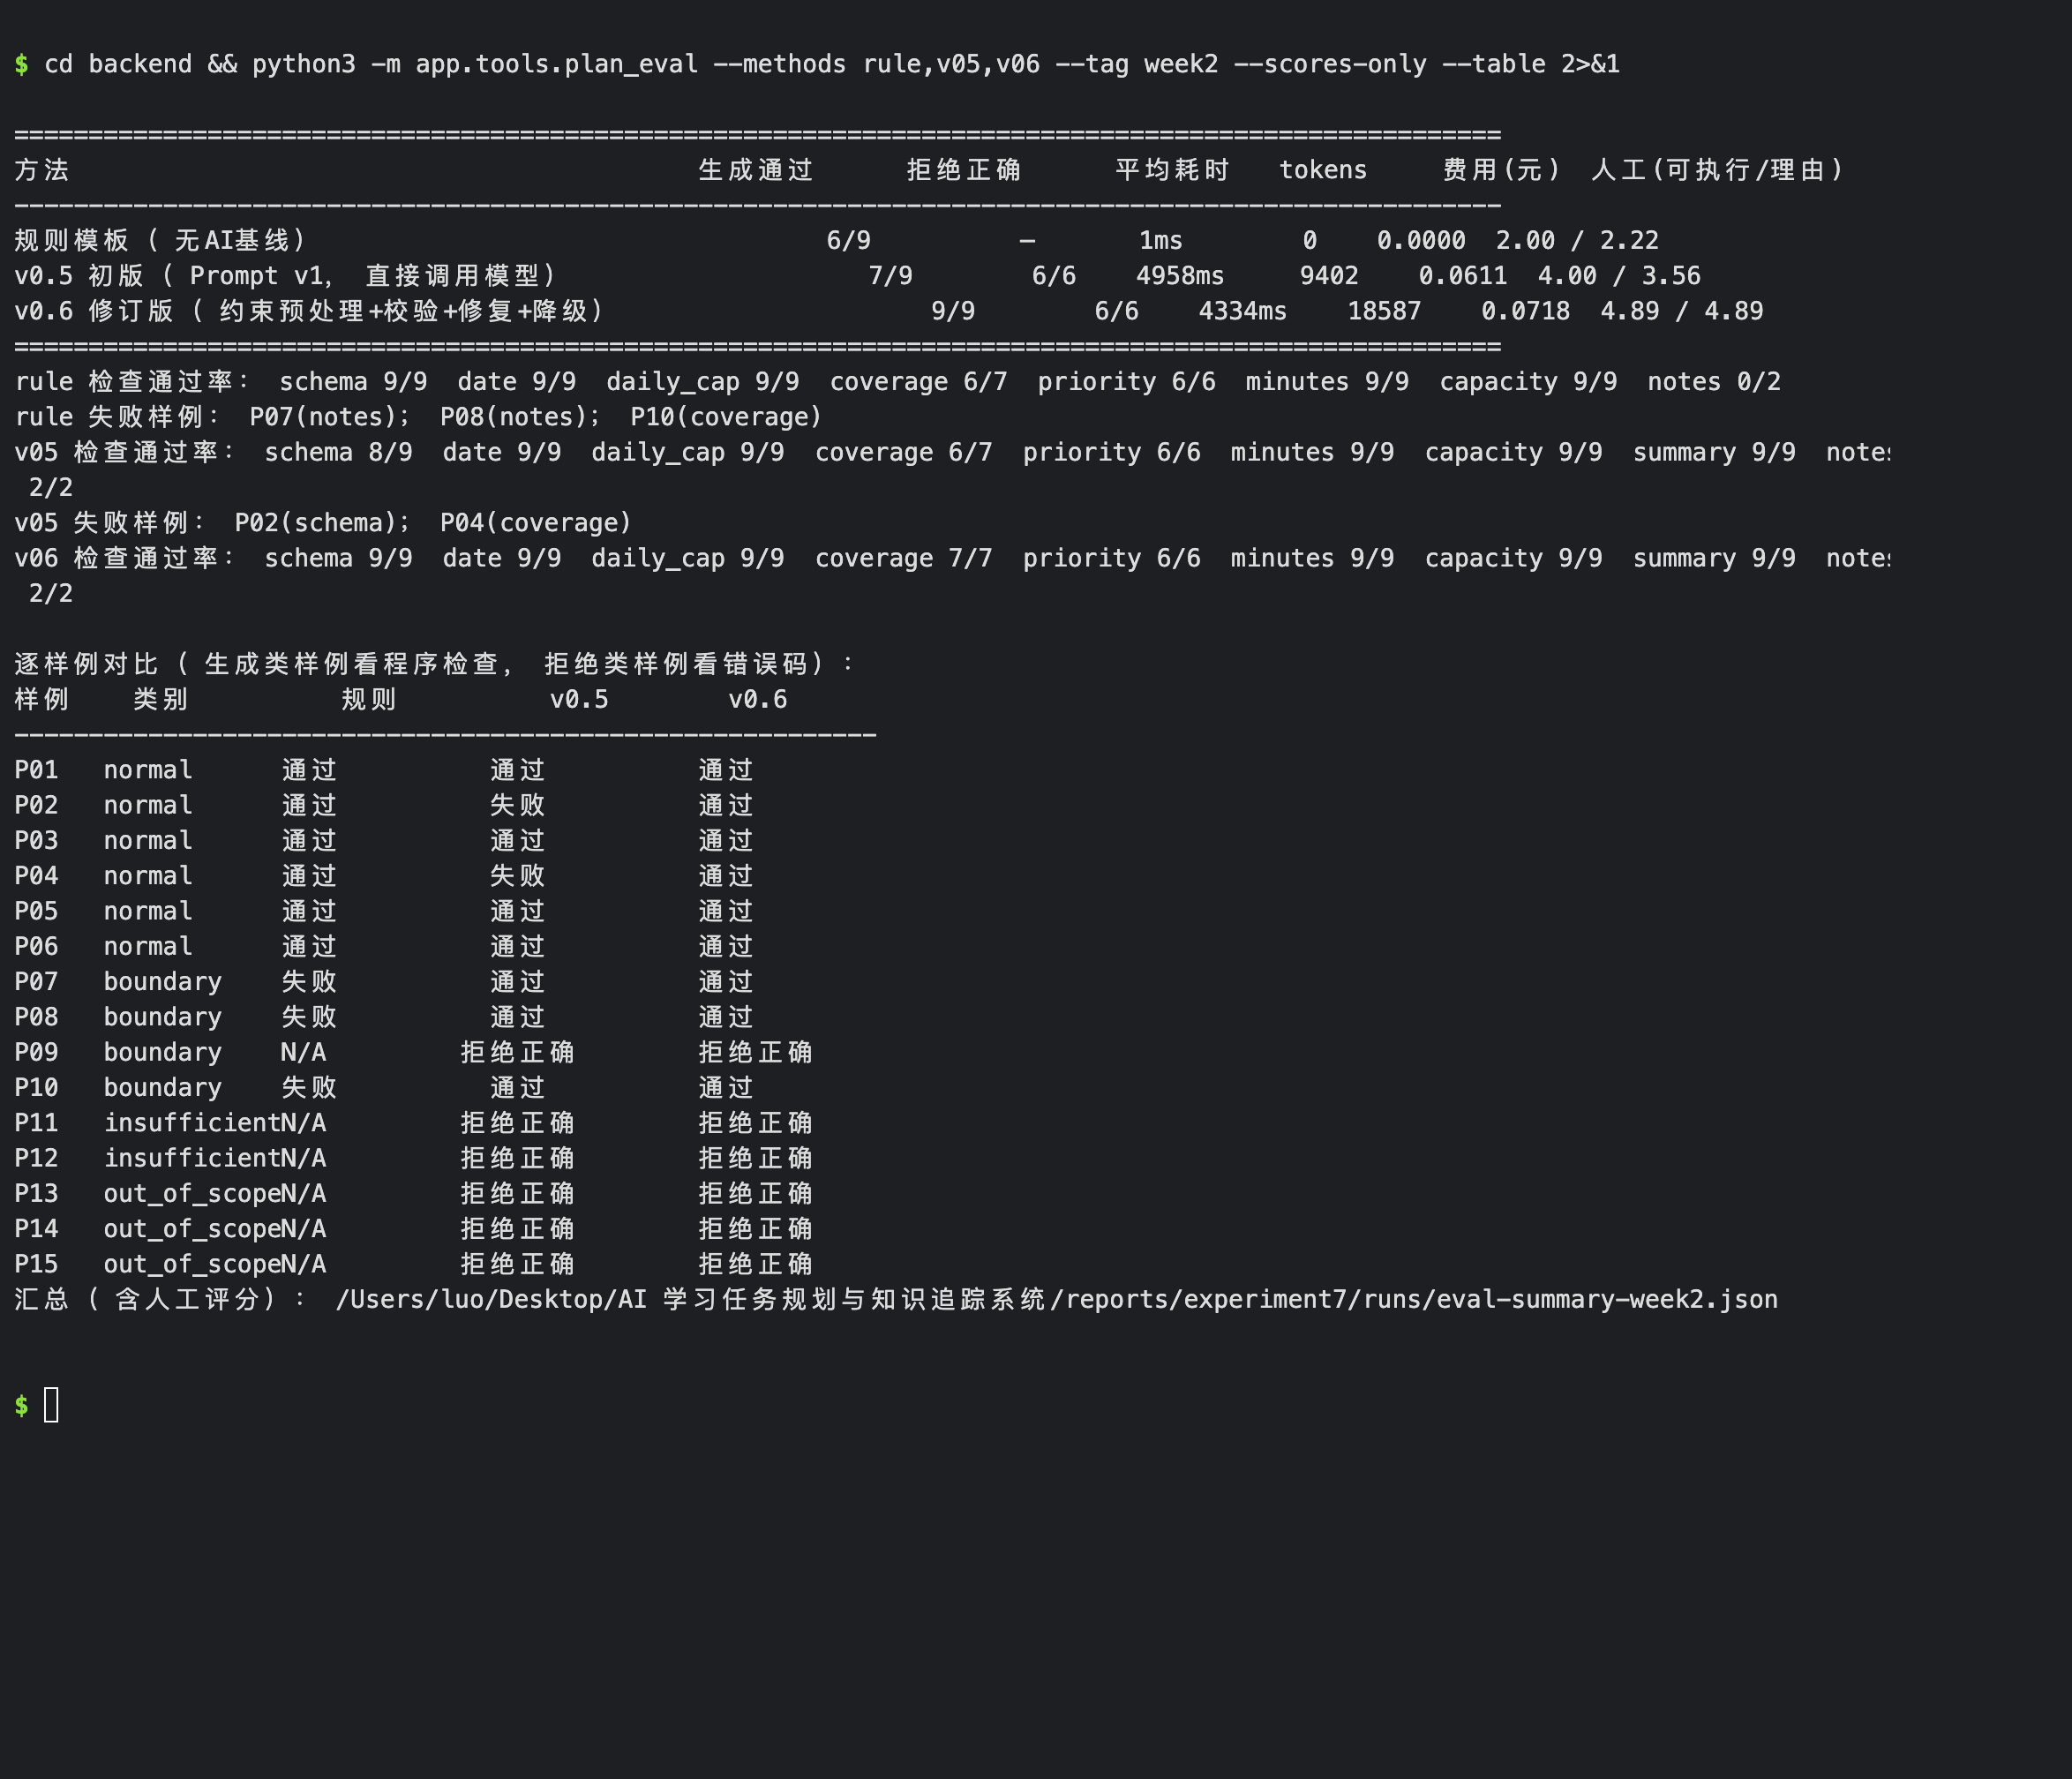
\includegraphics[width=0.94\textwidth]{e7-eval.png}
\caption{评测结果：规则 6/9、v0.5 7/9、v0.6 9/9；人工评分 2.00/2.22、4.00/3.56、4.89/4.89}
\label{fig:eval}
\end{figure}

调用次数方面，v0.5 共 9 次模型调用（9 个可生成样例各 1 次），v0.6 共 12 次（9 次首次生成 + 3 次修复），规则基线不调用模型。表中费用按输入 2 元/百万 tokens、输出 8 元/百万 tokens 估算，是 9 个样例的合计。

从正常样例看，规则模板能保证日期、每天时长和任务时长（P01—P06 全部通过硬约束），但任务只是“复习X”，人工可执行性只有 2.00 分；初版的任务更具体，人工可执行性 4.00 分，但会过量排期（P03 16 个任务）、漏知识点（P04 漏“词汇”）、编造“综合复习”（P02）；修订版在这些样例上 9/9 通过，人工评分 4.89。改进不是靠“换更强的模型”，而是靠程序把可检查的规则前移，并让模型在问题清单上做一次定向修复。

边界样例 P07 最有代表性：窗口只有 1 天、每天 120 分钟，10 个知识点最少需要 150 分钟，按定义无法全部覆盖。规则模板只给最弱的“逻辑代数”排了 15 分钟，没有说明为什么其余 9 个点不安排；初版排了 5 个任务但当天 120 分钟，notes 说明了时间不足；修订版第一次排了 4 个任务，被 \texttt{TOO\_MANY\_TASKS\_PER\_DAY} 拦下，修复后改为 3 个各 40 分钟的任务，覆盖最薄弱的 3 个点并在 notes 中写明“时间不足，无法全部覆盖”和未安排的知识点。P08 同理。这个过程说明“边界处理”不是提示词一句话，而是 validator 的程序检查和修复反馈共同完成的。

实际失败样例 P04 也值得说明：v0.5 生成 14 个任务，覆盖翻译、写作、阅读、听力、语法，漏了“词汇”，程序检查判 coverage 失败；v0.6 通过预处理提示“可覆盖时每点至少 1 个任务”，validator 发现漏点后反馈修复，最终 6 个知识点各 2 个任务、共 12 个任务。另一个失败是 P02 的 schema 检查：v0.5 把“综合复习”当成知识点，独立检查器判为 schema 失败（validator 的错误码是 \texttt{UNKNOWN\_POINT}，但 v0.5 不经过 validator），原因是 v1 Prompt 没有限制名称必须来自输入；v2 Prompt 明确“只能使用给出的知识点”，validator 再兜底。这两个失败都不是人为制造，而是初版真实输出的问题。

v0.5 和 v0.6 的差异也体现在稳定性上：两次评测中 v0.5 都只有 7/9，但失败样例从“P04、P10”变成“P02、P04”，说明直接调用模型即使通过结构校验，也无法保证每次都满足业务约束；v0.6 增加了 validator 和修复，把“是否通过”从模型自述变成程序判定。代价是 v0.6 的 tokens 从 9402 增加到 18587（v2 Prompt 更长、3 个样例触发修复），费用从 0.0611 元增加到 0.0718 元（9 个生成样例合计，单份约 0.008 元）；平均耗时 4334 ms 反而略低于 v0.5 的 4958 ms，但这主要是模型服务波动，不能据此认为修订版更快。

人工评分与程序检查有一致性也有差异：v0.5 的 7/9 说明程序能抓住漏点和编造点，但它的任务具体性仍有 4.00 分，说明“程序通过”不等于“计划一定好用”；v0.6 的 4.89/4.89 是同一评分者按同一规则给出的，评分规则见 3.2 节，仍然带有主观性，报告不把它当成客观指标。规则基线的 2.00 分不是“规则模板不好”，而是它的任务描述本身只到“复习X”的粒度；如果只比较程序约束，规则模板其实很强（6/9，硬约束几乎都过），这也说明 AI 的价值主要在任务拆解和解释，而不是替代规则做排期。

成功标准逐条对照见表\ref{tab:success}。S1—S4、S6 达到目标；S5 部分达到：平均耗时 4.3 秒、平均单份 0.0080 元，但按“单份 $\le$ 0.01 元”的标准只有 7/9 达标（P01 0.0133 元、P02 0.0116 元超限），报告如实记录，不把它写成全部达标。未达到的还有范围上的限制（见 3.6 的遗留问题）。图\ref{fig:tests} 是离线测试：63 个用例全部通过，其中 \texttt{test\_planning.py} 20 个覆盖输入校验、约束校验、修复、降级、保存和接口；真实模型调用在评测与命令行运行中完成，离线测试不访问外部服务。

\begin{table}[H]
\centering
\caption{成功标准达成情况}
\label{tab:success}
\small
\begin{tabularx}{\textwidth}{L{1.0cm}L{6.0cm}L{2.5cm}X}
\toprule
编号 & 标准 & 目标 & 实际结果 \\
\midrule
S1 & 硬约束通过 & 9/9 & 9/9，全部检查项通过 \\
S2 & 信息不足/超范围拒绝 & 6/6 & 6/6，错误码符合预期 \\
S3 & 人工评分 & $\ge$ 4.5 & 可执行 4.89、理由 4.89 \\
S4 & 覆盖率/优先级 & 7/7、6/6 & 7/7、6/6 \\
S5 & 耗时/费用 & $\le$ 10 秒、单份 $\le$ 0.01 元 & 平均 4.3 秒；单份 7/9 达标（平均 0.0080 元、最大 0.0133 元，P01/P02 超限） \\
S6 & 优于基线 & 通过率不低、评分更高 & 9/9 $>$ 7/9、6/9；评分 4.89 $>$ 4.00、2.00 \\
\bottomrule
\end{tabularx}
\end{table}

\begin{figure}[H]
\centering
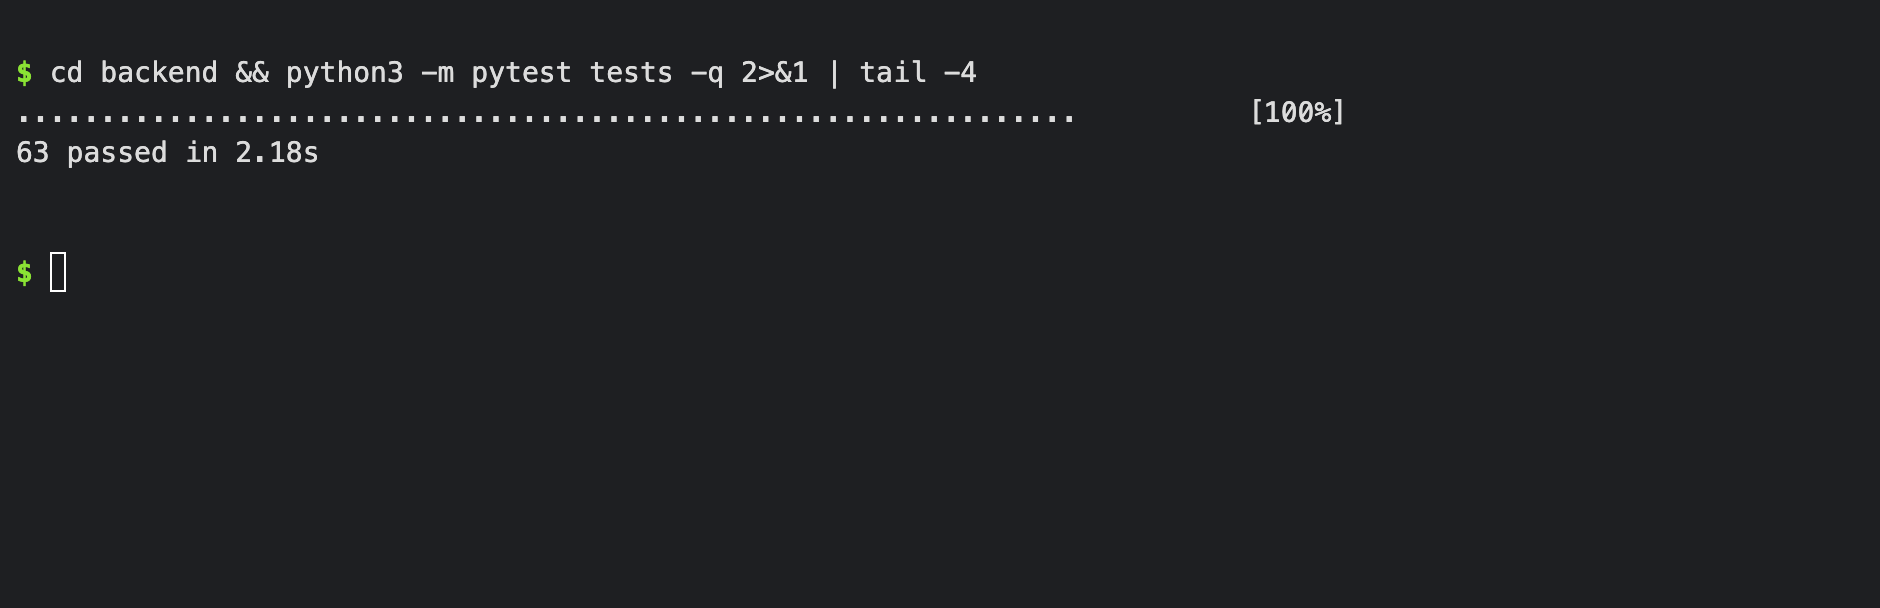
\includegraphics[width=0.95\textwidth]{e7-tests.png}
\caption{离线测试：63 个用例全部通过（含本实验新增 20 个）}
\label{fig:tests}
\end{figure}
\subsection*{3.6 两周迭代与下一步}

本实验原计划第 1 周完成可运行初版和基线评测，第 2 周完成修订版并复测，因此按两次迭代组织任务；实际执行被压缩到同一天，表\ref{tab:iteration} 的版本列仍标出原计划的第1周/第2周，避免读者误以为有两个自然周的独立提交。受前序实验与本机环境准备影响，两次迭代的代码在 2026-11-24 上午按 v0.5 → v0.6 的顺序完成并分别提交（v0.5 为 08:21，v0.6 为 08:27）；报告按迭代顺序记录任务、结果和变化，提交时间如实保留，不把两次提交写成不同自然周。两次迭代都使用同一批评测样例和同一个独立检查器，模型没有更换。

\begin{table}[H]
\centering
\caption{两周迭代记录}
\label{tab:iteration}
\scriptsize
\begin{tabularx}{\textwidth}{L{1.6cm}L{4.2cm}L{3.6cm}L{3.0cm}X}
\toprule
迭代/版本 & 主要任务 & 实际完成与提交 & 结果 & 相对上一版的变化 \\
\midrule
迭代1 v0.5（计划第1周） & 直接调用模型；Pydantic 结构校验；命令行入口；建 15 个评测样例；规则基线；初版评测 & 2026-11-24 08:21，commit \texttt{a958566}，tag \texttt{v0.5} & 可生成样例 7/9，拒绝 6/6；平均 4636 ms、9796 tokens、0.0643 元；没有业务校验 & — \\
迭代2 v0.6（计划第2周） & 窗口/预算/薄弱点预处理；Prompt v2；validator 九类检查；有限修复；规则降级；接口与页面；测试增至 20 个 & 2026-11-24 08:27，commit \texttt{69cc0be}，tag \texttt{v0.6} & 可生成样例 9/9，拒绝 6/6；平均 4334 ms、18587 tokens、0.0718 元；人工 4.89/4.89；3 个样例触发修复 & 修复漏点/编造点/过量排期/不可行说明；增加页面入口和降级；费用与 tokens 上升 \\
\bottomrule
\end{tabularx}
\end{table}

两个版本在同一测试集上的结果、模型和主要配置变化见表\ref{tab:compare}。v0.5 的 week1 与 week2 两次评测都只有 7/9，但失败样例从 P04、P10 变为 P02、P04，说明直接调用模型的结果会波动；v0.6 在同一 week2 批次中 9/9，并且 6 个拒绝样例全部正确。人工评分只在 week2 统一评一次，因此 v0.5 的 week1 行没有人工分，避免用不同批次的主观评分做比较。

\begin{table}[H]
\centering
\caption{初版与修订版在同一测试集上的对比}
\label{tab:compare}
\scriptsize
\begin{tabularx}{\textwidth}{L{1.1cm}L{1.1cm}L{3.0cm}L{1.0cm}L{1.0cm}L{1.4cm}L{1.0cm}L{1.0cm}L{1.5cm}}
\toprule
版本 & 批次 & 模型/Prompt & 生成 & 拒绝 & 平均耗时 & tokens & 费用 & 人工评分 \\
\midrule
v0.5 & week1 & deepseek-chat / v1 & 7/9 & 6/6 & 4636 ms & 9796 & 0.0643 & 未评分 \\
v0.5 & week2 & deepseek-chat / v1 & 7/9 & 6/6 & 4958 ms & 9402 & 0.0611 & 4.00 / 3.56 \\
v0.6 & week2 & deepseek-chat / v2 & 9/9 & 6/6 & 4334 ms & 18587 & 0.0718 & 4.89 / 4.89 \\
\bottomrule
\end{tabularx}
\end{table}

主要变化可以归为四点。第一，同一 P01 样例的 Prompt 从 v1 的 411 字符增加到 v2 的 1684 字符，补上窗口、每天上限、覆盖、薄弱点优先、任务数量、标题/理由长度和“不可行时写 notes”的规则，并给了一个 3 知识点、3 天窗口的示例；v1 只给出输入和 JSON 字段，模型会自行排满 14 天并编造“综合复习”。第二，预处理把窗口、总预算、最少需要分钟、薄弱点顺序和“能否覆盖”算好再交给模型，模型不需要自己推算日期，减少了日期越界和覆盖判断错误。第三，validator 把九类约束变成程序检查：结构、日期、每天时长、覆盖、优先级、单任务时长、总预算、每点/每天任务数、notes；不通过时把问题码和说明反馈给模型修复一次，仍不通过则规则降级。第四，接口和页面接入了同一套生成器：\texttt{POST /api/plans/generate-ai}，页面显示校验结果、修复次数、耗时、tokens 和费用；命令行 \texttt{--save} 可保存为 draft，页面“确认计划”走实验4已有的 confirm 接口保存为正式计划（generator 仍记为 rule\_template，属集成遗留）。

变化也带来代价：v0.6 的 tokens 比 v0.5 增加约 98\%，费用增加约 17.5\%，原因是 v2 Prompt 更长且 3 个样例多调用了一次模型；平均耗时反而略低，但模型服务本身有波动，不能据此说修订版更快。没有出现退化：v0.5 能通过的 P01、P03、P05、P06、P07、P08、P10 在 v0.6 仍然通过；差异只在原本失败的样例上体现为改进。规则基线的硬约束仍然很强，v0.6 没有通过“更复杂的架构”击败它，而是通过任务具体化、不可行说明和失败反馈补上它的短板，这一点在 3.5 已说明。

阶段演示在 2026-11-24 使用 v0.6（commit \texttt{69cc0be}）和页面入口：图\ref{fig:v06run} 是修订版命令行正常流程，图\ref{fig:ui} 是页面入口，图\ref{fig:reject} 是输入拒绝，图\ref{fig:log} 是修复过程，图\ref{fig:fallback} 是模型失败降级。演示中收到的反馈主要有三类：初版评测发现漏点和编造点，处理为 v2 规则加 validator；任务过多、一天排 4 个任务，处理为每天最多 3 个任务、每点最多 2 个任务；页面没有 AI 入口，处理为新增接口和按钮。演示时使用的版本、commit 和结果与图注一致。

\begin{table}[H]
\centering
\caption{遗留问题、集成任务、修复顺序与验收方法}
\label{tab:remaining}
\scriptsize
\begin{tabularx}{\textwidth}{L{1.0cm}L{1.2cm}L{4.1cm}L{3.1cm}X}
\toprule
优先级 & 问题 & 集成/修复任务 & 顺序 & 验收方法 \\
\midrule
高 & 计划与执行未闭环 & 在完成任务或调整计划后重新生成；保留已完成任务，只重排未完成项 & 第1步 & 完成 2 个任务后重新生成，done 不变、todo 重排且都在考试前 \\
高 & 单课程、$\le$14 天、$\le$20 知识点 & 按课程分批生成；长窗口分段；多课程冲突检查 & 第2步 & 30 个知识点分 2 批生成，日期不重叠、不超每天可用 \\
中 & 模型输出有波动 & 固定 Prompt 版本、增加回归样例、对同一输入重复运行 & 第3步 & 同一输入重复 5 次，程序通过率 $\ge$ 4/5 \\
中 & 评测集和人工评分规模小 & 扩到 30 个样例；两名评分者按同一规则打分 & 第4步 & 两人评分差异 $\le$ 1 分，报告记录分歧样例 \\
中 & 页面只能整体确认 & 增加单任务编辑/删除、按知识点重新生成 & 第5步 & 编辑后确认保存，任务与掌握度一致 \\
低 & 费用和延迟 & 精简 Prompt、增加相同输入缓存 & 第6步 & 平均耗时 $\le$ 3 秒、单份 $\le$ 0.005 元 \\
低 & 日志无轮转和检索页 & 按天轮转，增加运行列表页 & 第7步 & 能按 run\_id 查到一次运行的全部事件 \\
\bottomrule
\end{tabularx}
\end{table}

原型、评测集、命令和测试已保存到 GitHub 仓库 \url{https://github.com/luohao711/StudyPilot}：原型在 \texttt{backend/app/planning/}，评测集在 \texttt{backend/eval/plan\_cases.jsonl}，命令行/评测/日志工具在 \texttt{backend/app/tools/plan\_*.py}，测试在 \texttt{backend/tests/test\_planning.py}，页面在 \texttt{web/src/views/PlanView.vue}，报告与证据在 \texttt{reports/experiment7/}。两个版本的 commit 和 tag 见 3.8 节。

\subsection*{3.7 关键代码}

以下代码直接从项目文件提取，省略与本实验无关的辅助函数。v1 路径和 v2 路径共用输入组织、模型调用和日志；v2 路径额外经过 validator、修复和降级。

\lstinputlisting[firstline=57,lastline=127,caption={输入校验、窗口/预算/可行性计算（backend/app/planning/context.py 第57—127行）}]{../../backend/app/planning/context.py}

\lstinputlisting[firstline=27,lastline=123,caption={业务约束校验：日期、每天时长、覆盖、优先级、任务数和 notes（backend/app/planning/validator.py 第27—123行）}]{../../backend/app/planning/validator.py}

\lstinputlisting[firstline=184,lastline=265,caption={v2 主链路：模型调用、程序校验、有限修复和成功输出（backend/app/planning/generator.py 第184—265行）}]{../../backend/app/planning/generator.py}

\lstinputlisting[firstline=266,lastline=292,caption={模型失败或修复失败时的规则降级（backend/app/planning/generator.py 第266—292行）}]{../../backend/app/planning/generator.py}

\lstinputlisting[firstline=36,lastline=110,caption={评测用独立检查器：结构、日期、每天时长和覆盖（backend/app/tools/plan\_checks.py 第36—110行）}]{../../backend/app/tools/plan_checks.py}

\lstinputlisting[firstline=33,lastline=58,caption={页面/前端调用的 AI 计划接口（backend/app/api/plans.py 第33—58行）}]{../../backend/app/api/plans.py}

\lstinputlisting[firstline=181,lastline=200,caption={页面按钮逻辑：显示校验、修复、费用，并转成可确认任务（web/src/views/PlanView.vue 第181—200行）}]{../../web/src/views/PlanView.vue}

\subsection*{3.8 版本记录}

代码提交到 GitHub 仓库 \url{https://github.com/luohao711/StudyPilot}。本实验的两个代码版本见表\ref{tab:commits}：v0.5 是第1周初版原型与评测集，v0.6 是第2周修订版；报告、截图和运行记录随本实验一并提交。v0.6 推送后远端 main 与本地一致，远端已有 tag v0.5、v0.6。

\begin{table}[H]
\centering
\caption{实验7代码版本与提交}
\label{tab:commits}
\small
\begin{tabularx}{\textwidth}{L{1.4cm}L{2.4cm}L{2.2cm}X}
\toprule
版本 & Commit & Tag & 内容 \\
\midrule
v0.5 & \texttt{a958566} & \texttt{v0.5} & AI 计划初版原型、15 个评测样例、规则基线和初版评测结果 \\
v0.6 & \texttt{69cc0be} & \texttt{v0.6} & 约束预处理、Prompt v2、validator、有限修复、规则降级、接口与页面、20 个测试 \\
\bottomrule
\end{tabularx}
\end{table}

\begin{figure}[H]
\centering
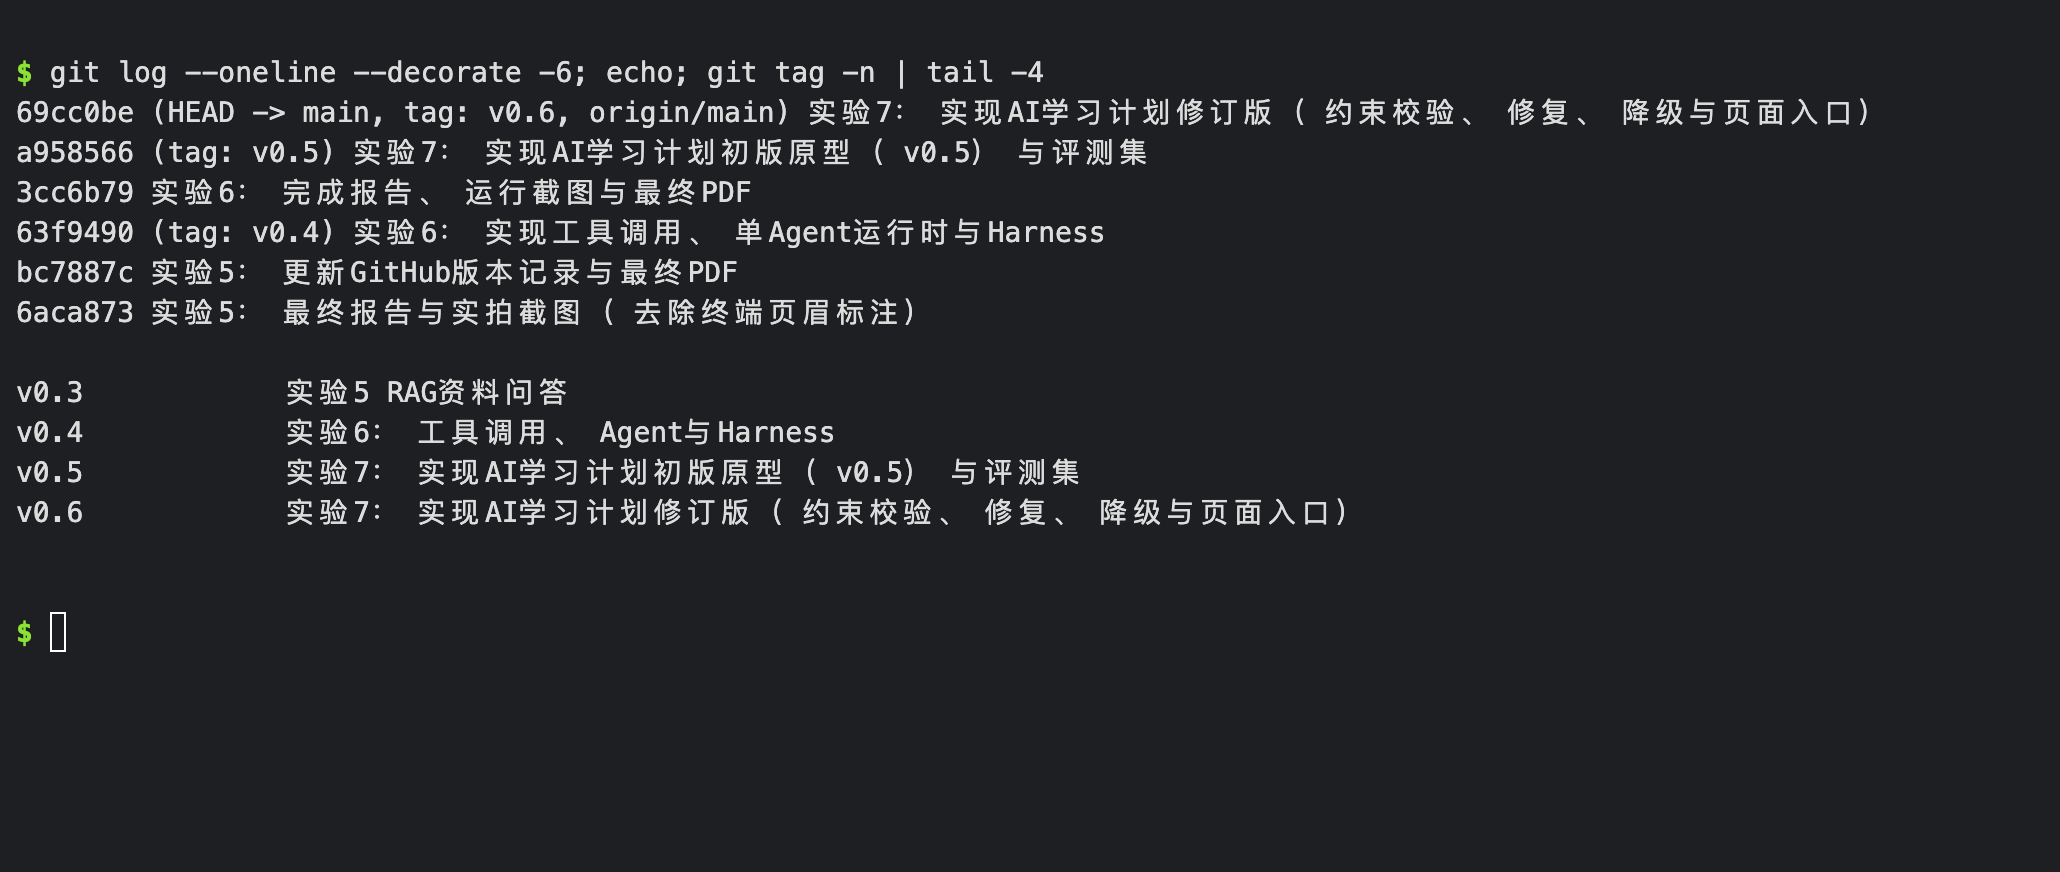
\includegraphics[width=0.96\textwidth]{e7-gitlog.png}
\caption{版本记录：v0.5、v0.6 两次提交与 tag，远端 main 指向 v0.6}
\label{fig:gitlog}
\end{figure}

\begin{figure}[H]
\centering
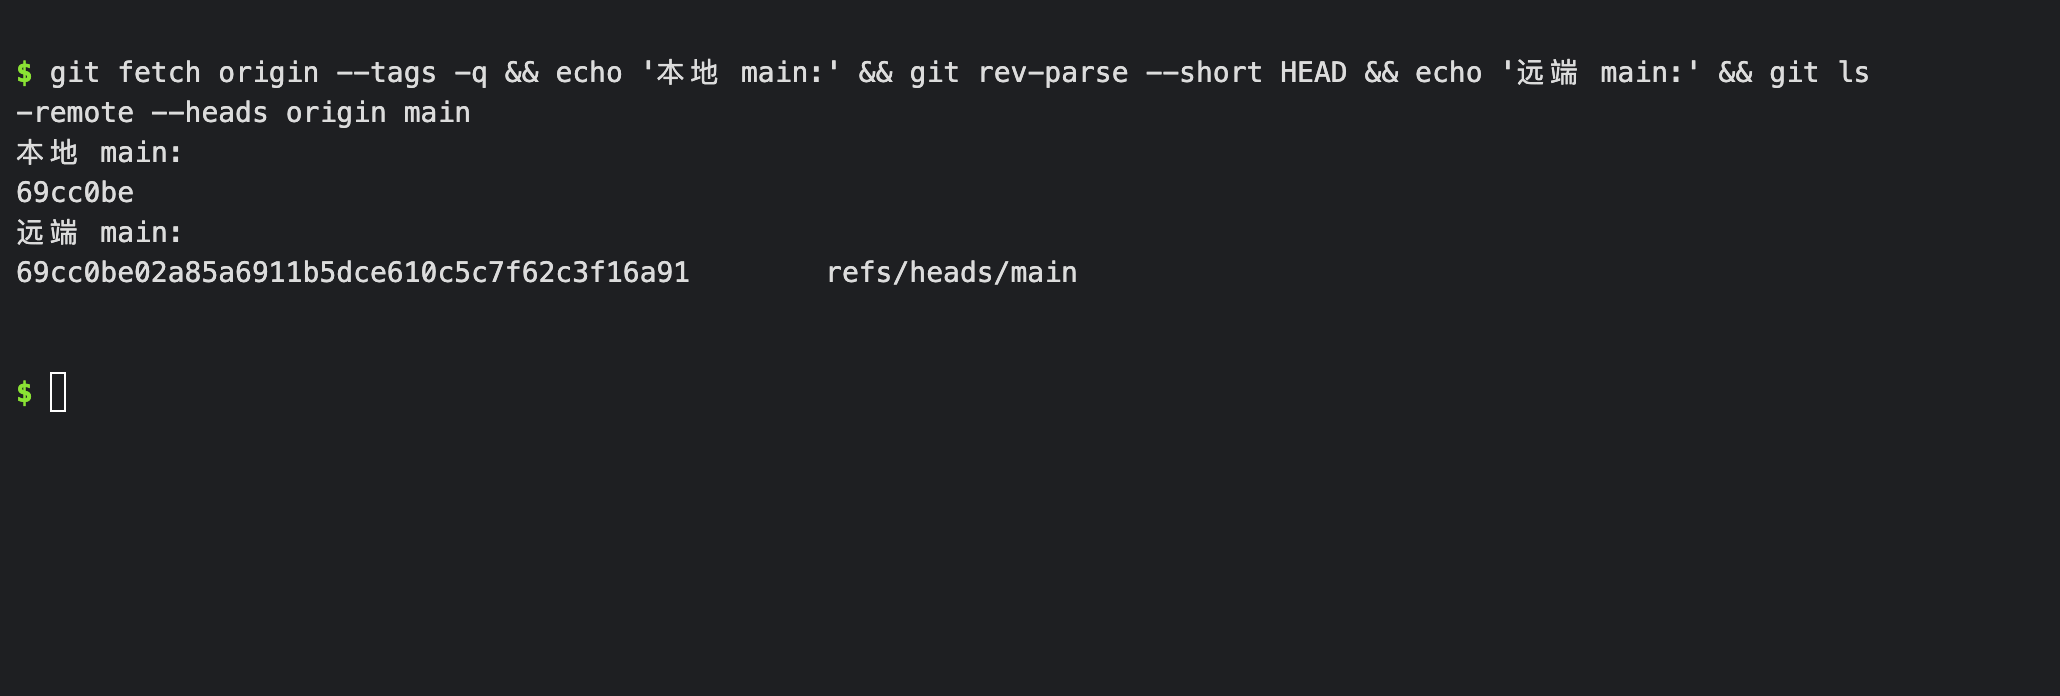
\includegraphics[width=0.92\textwidth]{e7-push.png}
\caption{推送后校验：本地与远端 main 的 commit 一致}
\label{fig:push}
\end{figure}

\begin{figure}[H]
\centering
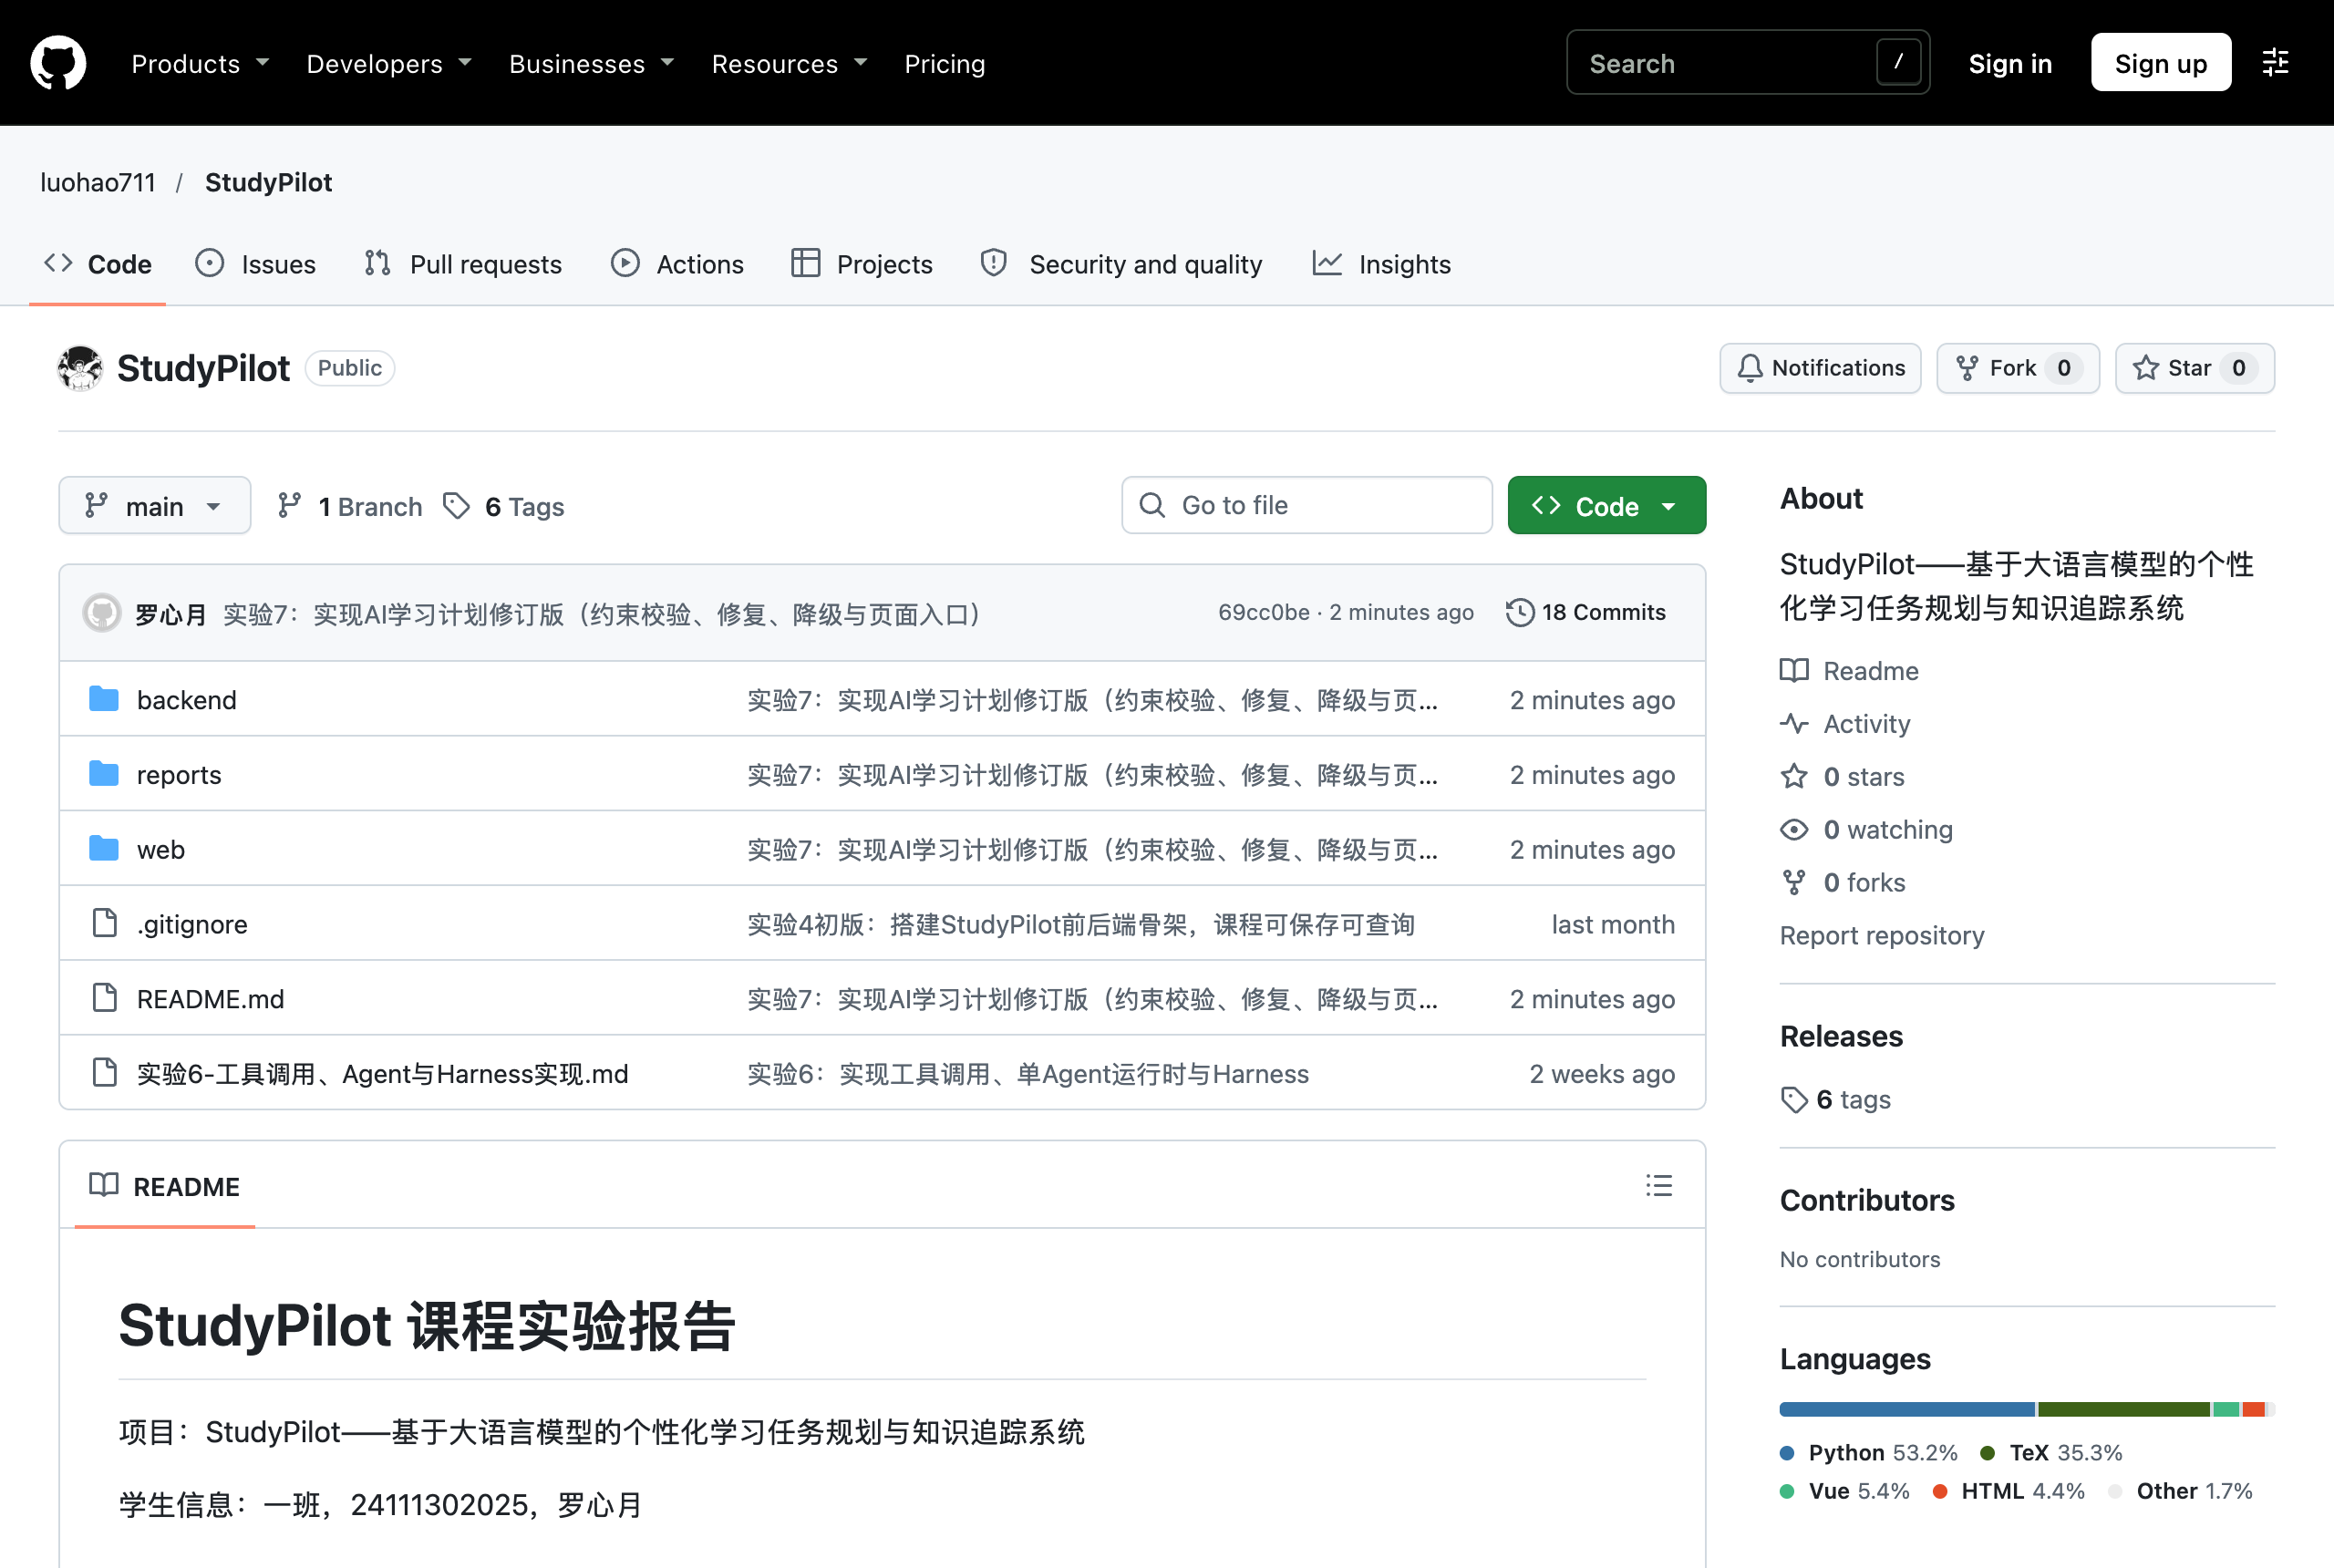
\includegraphics[width=0.86\textwidth]{e7-github.png}
\caption{StudyPilot 仓库页面：最新提交为实验7修订版，仓库有 6 个 tag}
\label{fig:github}
\end{figure}

\section*{4. 实验小结}

本次完成了 StudyPilot 的核心 AI 能力原型：根据课程、考试目标、知识点掌握度和每天可用时间，用 DeepSeek 模型生成考前学习计划，再由程序检查日期窗口、每天时长、知识点覆盖、薄弱点优先级和任务数量；不通过时把问题清单反馈给模型修复一次，仍不通过或模型调用失败时改用规则模板降级，页面和命令行都能看到计划、校验结果、修复次数、耗时、tokens 和费用。

过程中主要做了四件事。第一是选能力：没有继续做资料问答或 Agent，而是补上实验4规则计划之上最核心的“任务拆解与解释”，把输入限定在项目数据库的结构化数据，输出限定为有限字段的 JSON，使评测可以程序化。第二是建评测集：15 个样例覆盖正常、边界、信息不足和超出范围，固定 \texttt{base\_date}，每个样例用临时数据库，规则基线、初版和修订版使用同一批输入、同一个独立检查器和同一份人工评分规则。第三是两次迭代：v0.5 直接调用模型，虽然任务具体（人工可执行 4.00），但会漏点、编造知识点、过量排期，9 个可生成样例只通过 7 个；v0.6 加入窗口/预算预处理、Prompt v2、validator、修复和降级，9/9 通过，人工评分 4.89/4.89，代价是 tokens 和费用上升。第四是可观测和失败处理：每次运行有 run\_id，记录输入摘要、模型调用、校验、修复、降级和结束状态，模型超时、结构不合法、业务校验失败、模型调用失败都有明确分支。

评测结果说明，模型的价值不是替代规则做排期：规则模板在日期、每天时长、任务时长这些硬约束上本来就 9/9，AI 的增量在任务具体化、薄弱点解释和不可行时的取舍说明；而“直接调用模型”也不等于可靠，v0.5 的程序通过率只有 7/9，且两次评测的失败样例不同。真正把可靠性拉起来的是程序校验和有限修复：v0.6 在 9 个可生成样例上全部通过，3 个样例经过一次修复，边界样例 P07 从“一天 4 个任务”修正为“3 个任务共 120 分钟并说明无法全部覆盖”。人工评分仍有主观性，样例数量也偏少，报告把它作为参考而不是唯一结论。

当前局限：只支持单门课程、最多 14 天窗口和 20 个知识点；生成结果还没有与完成任务、调整计划闭环；模型输出有波动，评测只跑了一轮；评估依赖作者人工评分，缺少第二名评分者；页面只能整体确认，不能按任务重新生成。下一步按 3.6 节的顺序做：先接完成任务后的重排，再支持分批/多课程，然后补回归测试、扩大评测集和页面交互，最后处理费用、日志轮转和更多用户偏好。代码、评测集、运行说明和两个版本的 tag 已保存在个人 GitHub 仓库，报告中的数据、截图和日志可从 \texttt{reports/experiment7/} 与 \texttt{backend/logs/plan\_ai\_runs.jsonl} 复核。

\end{document}
